% PAKETE UND DOKUMENTKONFIGURATION
\documentclass[11pt, a4paper]{article}

% Encoding für Umlaute
\usepackage[utf8]{inputenc}
\usepackage[T1]{fontenc}

% Silbentrennung
\usepackage[ngerman]{babel}

% erweiterte Matheumgebungen und Formelnummer mit Sectionnummer
\usepackage{amsmath}
\numberwithin{equation}{section}

% Braket Notation
\usepackage{braket}

% zusätzliche mathematische Schriftarten
\usepackage{amsfonts}

% verschiedene mathematische Symbole
\usepackage{amssymb}

% Einheiten setzen z.B. \SI{10}{\kilo\gram\meter\per\second\squared}
% Fehler: \SI{10 +- 0,2e-4}{\metre}
\usepackage{siunitx}
\sisetup{
  output-decimal-marker={,},
  separate-uncertainty
}

% Randbreiten
\usepackage[left=3.5cm,right=3.5cm,top=3cm,bottom=3cm,twoside]{geometry}

% Bilder einfügen
\usepackage{graphicx}

% Verweise innerhalb des Dokuments
\usepackage{hyperref}
\hypersetup{
	colorlinks = true,
	allcolors = {black}
}

% bessere Tabellenlayouts
\usepackage{booktabs}
\usepackage{multirow}

% Seitenlayout (Kopfzeile)
\usepackage{fancyhdr}

% Float Barriers
\usepackage{placeins}

% Pakete für gedrehte Subfigures
\usepackage{caption}
\usepackage{subcaption}
\usepackage{rotating}

% Caption-Setup
\captionsetup{font={small}}
\renewcommand{\thefigure}{\thesection.\arabic{figure}}
\renewcommand{\thesubfigure}{\alph{subfigure}}
\renewcommand{\thetable}{\thesection.\arabic{table}}
\renewcommand{\thesubtable}{\alph{subtable}}

% Manuelle Silbentrennung
\hyphenation{Halb-werts-brei-te Fa-bry-Pé-rot-E-ta-lon Zee-man-E-ffekt Cad-mi-um-Lam-pe Kon-den-sor-lin-se}

% Tiefe des Inhaltsverzeichnisses (Level: 1 sections, 2 subsections,
% 3 subsubsections)
\setcounter{tocdepth}{3}

% FANCYHDR SETUP
\pagestyle{fancy}
\fancyhead[EL,OR]{\thepage}
\fancyhead[ER]{\leftmark}
\fancyhead[OL]{\rightmark}

\renewcommand{\sectionmark}[1]{
\markboth{Abschnitt \thesection{}: #1}{\thesection{} #1}
}
\renewcommand{\subsectionmark}[1]{
\markright{\thesubsection{} #1}
}

% DOKUMENTINFORMATIONEN
\title{P402 \\ Quantelung von Energie}

\author{Christopher Deutsch\footnote{christopher.deutsch@uni-bonn.de} \and Christian Bespin\footnote{christian.bespin@uni-bonn.de}}

\date{\today}

\begin{document}

\begin{titlepage}

\maketitle

% DURCHFÜHRUNGSDATUM UND ASSISTENT
\begin{center}
\begin{tabular}{l r}
Durchführung: & 1./2. Dezember 2014 \\
Gruppe: & $\alpha$ 2 \\
Assistent: & Dennis Sauerland
\end{tabular}
\end{center}

% ZUSAMMENFASSUNG
\begin{abstract}
\noindent

\end{abstract}

\end{titlepage}

% INHALTSVERZEICHNIS
\tableofcontents
% Neue Seite nach TOC
\newpage

% INHALT VERSUCHSPROTOKOLL

\section{Grundlagen / Theorie}

\subsection{Photoelektrischer Effekt}
Photoeffekt umfasst drei verschiedene Arten der Wechselwirkung von Licht mit Materie.
Betrachtet wird der äußere photoelektrische Effekt, das heißt das Herauslösen von Elektronen aus Metalloberflächen (oder Halbleiter) durch Photonen.
Erstmalige Deutung ("Licht" gibt Energie in Paketen welche Photonen genannt werden ab) von Einstein 1905 (Nobelpreis).
Energie eines Photons:
\begin{align}
	E_\gamma = h \cdot \nu
\end{align}




\subsection{Photozelle}

\subsubsection{Aufbau und Wirkung}
Photozelle: eine Form von Elektronenröhre
Zwei Elektroden im evakuierten Glaskolben (freie Weglänge $\Lambda$).
Elektroden: Photokathode (hierauf treffen die Photonen) und Anode (die hier aufgefangenen Elektronen verursachen den Photostrom).

Messung: Intensitäten oberhalb einer Grenzfrequenz (Austrittsarbeit);

Betriebsmodi: Saugspannung (Anode + Kathode -) oder Gegenspannung (Anode - Kathode +).


Elektronen in der Photokathode absorbieren Photonen der Energie $E_\gamma$.
Ist die Energie der Elektronen anschließend hoch genug (größer als die Austrittsarbeit), so können die Elektronen aus dem Metall austreten.
Die Energiebilanz des gelösten Elektrons (ohne Messkreis):
\begin{align}
E_e = E_\gamma - W_\mathrm{A} = h \cdot \nu - W_\mathrm{A}
\end{align}

\subsubsection{Photostromverlauf}

\begin{align}
	I_\mathrm{Photo} \propto (E_\mathrm{kin} - e \cdot U_0)^2
\end{align}

\subsubsection{Austrittsarbeit und Kontaktpotential}
Kontaktpotentialdifferenz zweier Metall ist gleich der Differenz ihrer Austrittsarbeiten (Der Photoeffekt Klaus/Herrmann)
Austrittsarbeit ist Abstand Fermi-Niveau - Kontinuum.
Bringt man zwei unterschiedliche Leiter mit verschiedenen Austrittsarbeiten in Kontakt, so entsteht ein Ladungsfluss der die Fermi-Niveaus beider Leiter ausgleicht.

\begin{align}
	U_\mathrm{K} = \frac{\phi_1 - \phi_2}{e}
\end{align}

\section{Bestimmung des Planckschen Wirkungsquantums}

\subsection{Durchführung}

\subsubsection{Aufbau und Justage}
\begin{figure}[h]
	\centering
	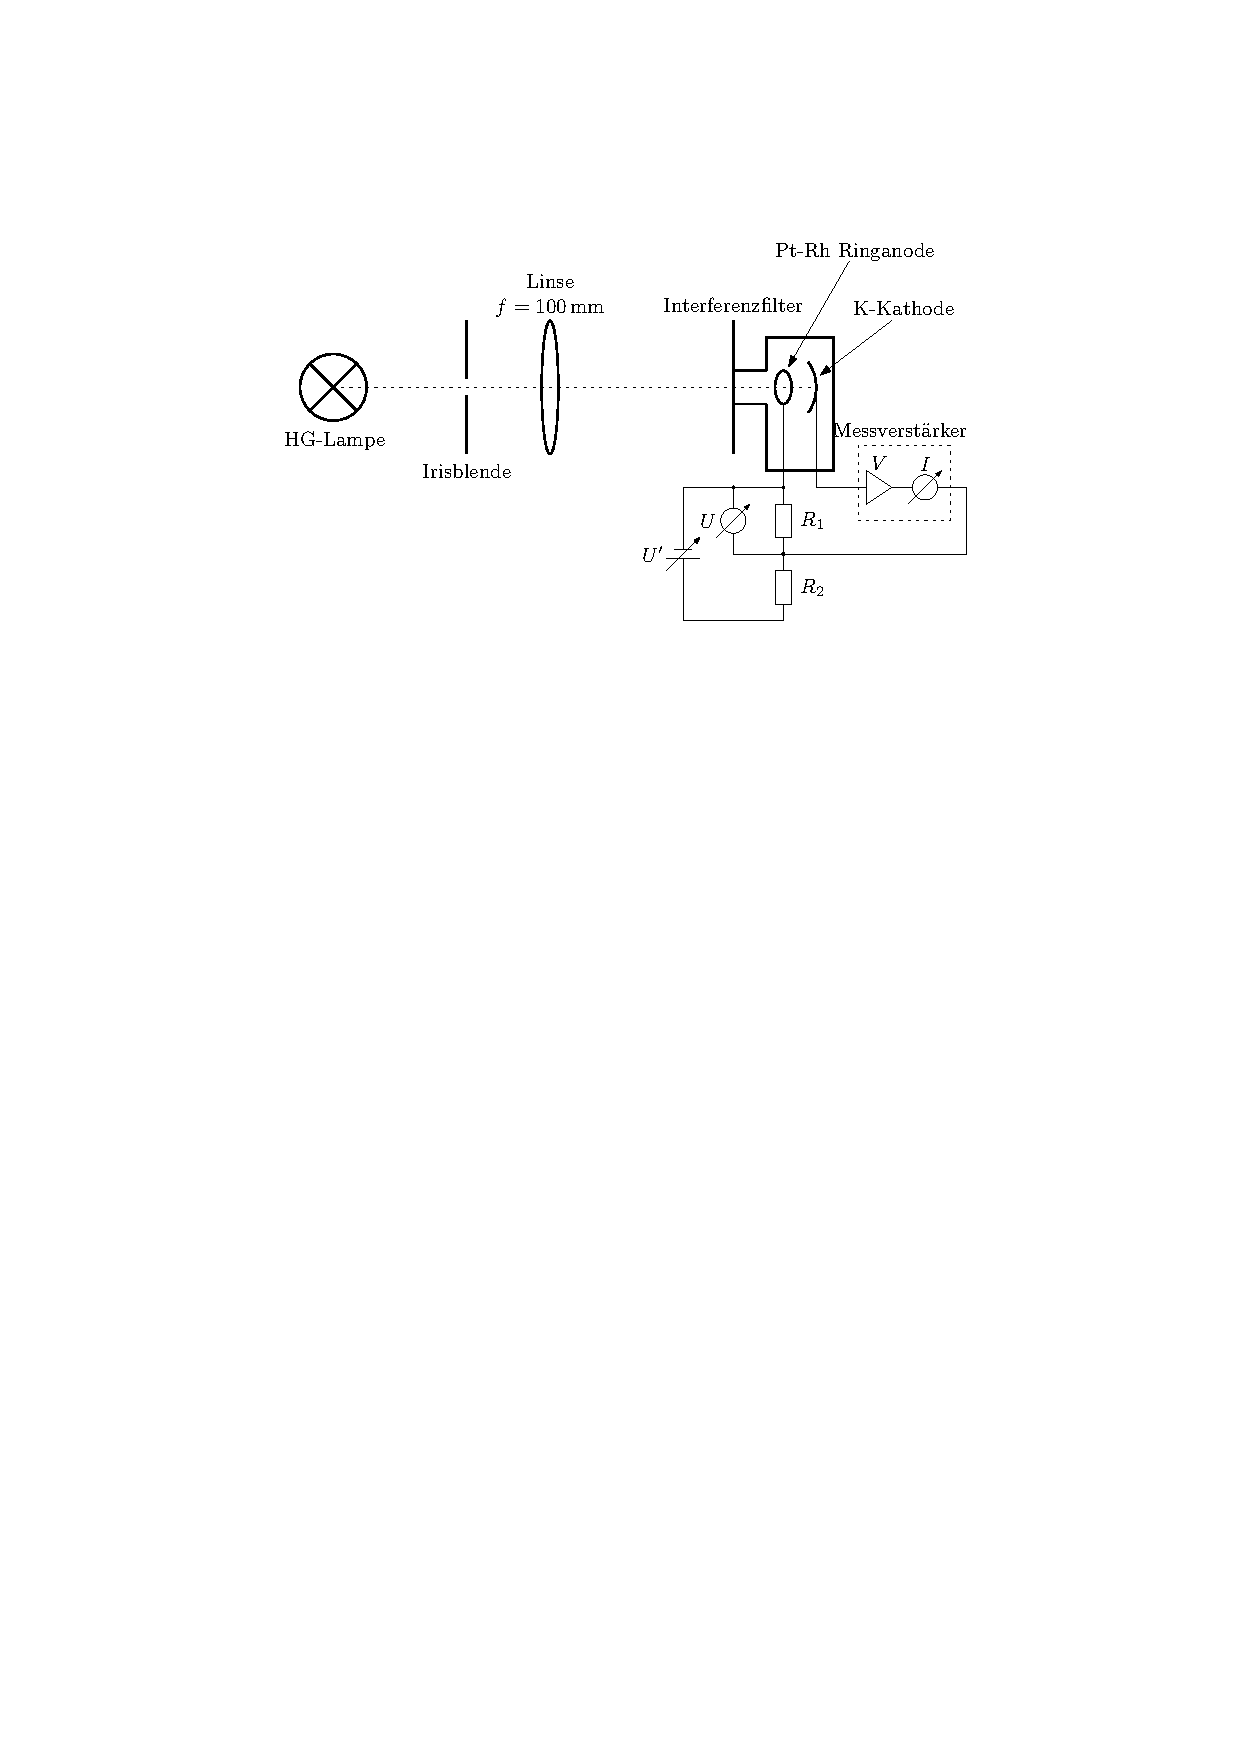
\includegraphics[width=0.9\textwidth]{./figures/versuchsaufbau_photoeffekt.pdf}
	\caption{Versuchsaufbau zur Bestimmung des Planckschen Wirkungsquantums durch den Photoeffekt}
	\label{fig:aufbau_photoeffekt}
\end{figure}
Um das Plancksche Wirkungsquantum zu bestimmen, ist es nötig die Photostrom-Gegenspannungs-Kennlinien $I$-$U$-Kennlinien einer Photozelle bei verschiedenen Wellenlängen $\lambda$ zu bestimmen.
Dazu verwenden wir zur Beleuchtung eine Quecksilberdampflampe, welche am Ende der optischen Bank befestigen.
Die vermessene Photozelle stellen wir am anderen Ende der Bank auf.
Um die Intensität des Lichts, welches in die Photozelle fällt regulieren zu können, wird vor die Lampe eine verstellbare Irisblende gestellt.
Zur Fokussierung des Lichts wird die Blende durch eine Linse ($f=\SI{100}{\milli\metre}$) auf die Kathode der Photozelle abgebildet.
Die Wellenlängenselektion erfolgt über ein Interferenzfilterrad, welches direkt vor die Photozelle gestellt wird.

Bei der Justage ist wichtig, dass alle Elemente auf einer optischen Achse liegen.
Dazu schalten wir die Lampe ein und nutzen die Reflexe von Linse und Interferenzfilter um alle Teile auf gleicher Höhe auszurichten.
Wir entfernen außerdem die Schutzkappe von der Photozelle und stellen die Linse so, dass die Blende scharf auf der Kathode abgebildet wird, wobei wir die Irisblende so einstellen, dass der Fleck einen Durchmesser von \num{5} bis \SI{10}{\milli\metre} hat.
Gleichzeitig nutzen wir diese Abbildung um die Höhe der Photozelle einzustellen, wobei wir beachten, dass die Anode nicht beleuchtet wird.
Nach dem Abschluss der Justage wird die Schutzkappe wieder auf die Photozelle gesetzt.

Die Elektronik zur Messung der Kennlinien besteht aus einer regelbaren Spannungsquelle (\num{0}-\SI{12}{\volt}), welche über einem Spannungsteiler die Gegenspannung der Photozelle liefert.
Zur Messung des Photostroms erfolgt über einen Messverstärker, welcher eine zum Strom proportionale Spannung ausgibt.
Die im Versuch auftretenden Ströme wurden dabei mit einem Verstärkungsfaktor von $V = \SI{1e-8}{\ampere\per\volt}$ gemessen, wobei der Fehler auf diesen vernachlässigt wird.
Die Messung von Gegenspannung und Photostrom erfolgt dann über zwei Voltmeter, welche die Spannung an Messverstärker beziehungsweise Spannungsteiler messen.

\subsubsection{Messung der Kennlinien}
Zunächst wählen wir den Interferenzfilter mit Mittenwellenlänge $\lambda = \SI{365}{\nano\metre}$ und überprüfen, in welcher Größenordnung sich die Grenzspannung $U_0$, bei der kein Photostrom mehr fließt, befindet.
Diese liegt in der Größenordnung von \SI{2}{\volt}, daher wählen wir einen Spannungsteiler aus \SI{100}{\ohm} und \SI{222}{\ohm}.
(Warum kein \SI{333}{\ohm ?})

Nun wird mit der Messung der Kennlinien für die Wellenlängen $\lambda = \num{365}$, \num{405} , \num{436}, \num{546}, \SI{578}{\nano\metre} begonnen.
Es wird für jeden Filter wie folgt vorgegangen:
\begin{itemize}
  \item Messung des Anodenphotostroms $I_0$: Es wird der Strom bei maximaler Gegenspannung gemessen, da bei dieser kein Kathodenphotostrom mehr stattfindet.
  Der gemessene Strom entspricht dabei nicht dem Anodenphotostroms, sondern der Summe von Anodenphotostrom und Offset des Verstärkers.
  Der Offset wurde nicht konkret bestimmt, da die gemessenen Kennlinien $I-I_0$ als Differenz zweier offsetbehafteter Größen aufgetragen werden und ein konstanter Versatz somit keinen Einfluss auf die Differenz hat. 
  \item Abschätzung der Grenzspannung $U_0$: Es wird die Gegenspannung langsam verringert bis ein signifikanter Anstieg des Photostroms beobachtet werden kann.
  Die Gegenspannung bei der dies einsetzt, dient als erste Abschätzung der Grenzspannung, so dass der Messbereich entsprechend gewählt werden kann.
  \item Messung der Kennlinie: Es wird bei der Messung bei einer Gegenspannung von $U = \SI{0}{\volt}$ begonnen, welche schrittweise bis zur abgeschätzten Grenzspannung $U_0$ hochgeregelt wird. Dabei wird beachtet, dass ausreichend Messpunkte im quadratischen Bereich der Kennlinie liegen.
\end{itemize}
Nachdem die Kennlinienmessung für jeden Filter einmal durchgeführt wurde, wiederholen wir die Messungen um Intensitätsschwankungen der Quecksilberdampflampe feststellen zu können.

Anschließend wird die Kennlinie der Photozelle bei höherer Intensität vermessen, dabei wird nur der Filter mit Mittelwellenlänge $\lambda = \SI{365}{\nano\metre}$ verwendet.
Dazu wird die Öffnung der Irisblende soweit vergrößert, dass ein signifikanter Anstieg des Photostroms beobachtet werden kann, ohne dabei die Ringanode zu beleuchten.
Analog zum vorigen Teil wird der Anodenphotostrom bei maximaler Gegenspannung gemessen, die Grenzspannung abgeschätzt und gemäß diesen der Messbereich der Kennlinie gewählt.

Es wird der absolute Fehler der Gegenspannungsmessung mit dem Digitalmultimeter konservativ auf $\Delta U = \SI{2}{\milli\ampere}$ abgeschätzt.
Im Gegensatz dazu, konnte eine starke Schwankung der Photostrom-Messung mit dem Messverstärker bei hohen Strömen festgestellt werden.
Daher wird hier ein relativer Fehler von $\frac{\Delta I}{I} = \SI{2}{\percent}$ abgeschätzt

\subsection{Auswertung}
Zunächst wird gemäß des Verstärkerfaktors von $V = \SI{1e-8}{\ampere\per\volt}$ aus der gemessenen Spannung der Photostrom $I$ und des Anodenstroms $I_0$ berechnet.
Es wird auf die Angabe der gemessenen Spannungen verzichtet und stattdessen direkt der Kathodenphotostrom $I-I_0$ angegeben.
Dabei wurde der Fehler $\Delta (I - I_0)$ durch Gaußssche Fehlerfortpflanzung aus den relativen Fehlern $\frac{\Delta I}{I} = \frac{\Delta I_0}{I_0} = \SI{2}{\percent}$ berechnet.
Die Kennlinienmessungen finden sich im Anhang \ref{app:kennlinien}.



\subsubsection{Bestimmung der Grenzspannung $U_0$ für die verschiedenen Wellenlängen}
\label{sssec:photoeffekt_grenzspannung}
Zur Bestimmung der Grenzspannung wird ausgenutzt, dass die Kennlinie im Anlaufgebiet quadratisch mit der Gegenspannung $U$ anwächst.
Daher kann durch Auftragen der Wurzel des Kathodenphotostroms $\sqrt{I-I_0}$ gegen die anliegende Gegenspannung $U$ die Kennlinie linearisiert werden und durch Extrapolation des linearen Teils der Kurve die Grenzspannung $U_0$ als Schnittpunkt mit der $x$-Achse berechnet werden.
Dabei ist zu beachten, dass bei hohen Gegenspannungen eine Abweichung vom quadratischen Zusammenhang zu beobachten ist, welche bei der Extrapolation vernachlässigt werden.
Die Linearisierung wurde in Abbildung \ref{fig:kennlinien_exemp_365nm} exemplarisch aufgetragen, wobei der Fehler gemäß der Gaußsschen Fehlerfortpflanzung bei Bildung der Wurzel berechnet wurde.
\begin{figure}[h]
	\centering
	% GNUPLOT: LaTeX picture with Postscript
\begingroup
  \makeatletter
  \providecommand\color[2][]{%
    \GenericError{(gnuplot) \space\space\space\@spaces}{%
      Package color not loaded in conjunction with
      terminal option `colourtext'%
    }{See the gnuplot documentation for explanation.%
    }{Either use 'blacktext' in gnuplot or load the package
      color.sty in LaTeX.}%
    \renewcommand\color[2][]{}%
  }%
  \providecommand\includegraphics[2][]{%
    \GenericError{(gnuplot) \space\space\space\@spaces}{%
      Package graphicx or graphics not loaded%
    }{See the gnuplot documentation for explanation.%
    }{The gnuplot epslatex terminal needs graphicx.sty or graphics.sty.}%
    \renewcommand\includegraphics[2][]{}%
  }%
  \providecommand\rotatebox[2]{#2}%
  \@ifundefined{ifGPcolor}{%
    \newif\ifGPcolor
    \GPcolortrue
  }{}%
  \@ifundefined{ifGPblacktext}{%
    \newif\ifGPblacktext
    \GPblacktexttrue
  }{}%
  % define a \g@addto@macro without @ in the name:
  \let\gplgaddtomacro\g@addto@macro
  % define empty templates for all commands taking text:
  \gdef\gplbacktext{}%
  \gdef\gplfronttext{}%
  \makeatother
  \ifGPblacktext
    % no textcolor at all
    \def\colorrgb#1{}%
    \def\colorgray#1{}%
  \else
    % gray or color?
    \ifGPcolor
      \def\colorrgb#1{\color[rgb]{#1}}%
      \def\colorgray#1{\color[gray]{#1}}%
      \expandafter\def\csname LTw\endcsname{\color{white}}%
      \expandafter\def\csname LTb\endcsname{\color{black}}%
      \expandafter\def\csname LTa\endcsname{\color{black}}%
      \expandafter\def\csname LT0\endcsname{\color[rgb]{1,0,0}}%
      \expandafter\def\csname LT1\endcsname{\color[rgb]{0,1,0}}%
      \expandafter\def\csname LT2\endcsname{\color[rgb]{0,0,1}}%
      \expandafter\def\csname LT3\endcsname{\color[rgb]{1,0,1}}%
      \expandafter\def\csname LT4\endcsname{\color[rgb]{0,1,1}}%
      \expandafter\def\csname LT5\endcsname{\color[rgb]{1,1,0}}%
      \expandafter\def\csname LT6\endcsname{\color[rgb]{0,0,0}}%
      \expandafter\def\csname LT7\endcsname{\color[rgb]{1,0.3,0}}%
      \expandafter\def\csname LT8\endcsname{\color[rgb]{0.5,0.5,0.5}}%
    \else
      % gray
      \def\colorrgb#1{\color{black}}%
      \def\colorgray#1{\color[gray]{#1}}%
      \expandafter\def\csname LTw\endcsname{\color{white}}%
      \expandafter\def\csname LTb\endcsname{\color{black}}%
      \expandafter\def\csname LTa\endcsname{\color{black}}%
      \expandafter\def\csname LT0\endcsname{\color{black}}%
      \expandafter\def\csname LT1\endcsname{\color{black}}%
      \expandafter\def\csname LT2\endcsname{\color{black}}%
      \expandafter\def\csname LT3\endcsname{\color{black}}%
      \expandafter\def\csname LT4\endcsname{\color{black}}%
      \expandafter\def\csname LT5\endcsname{\color{black}}%
      \expandafter\def\csname LT6\endcsname{\color{black}}%
      \expandafter\def\csname LT7\endcsname{\color{black}}%
      \expandafter\def\csname LT8\endcsname{\color{black}}%
    \fi
  \fi
  \setlength{\unitlength}{0.0500bp}%
  \begin{picture}(6480.00,4320.00)%
    \gplgaddtomacro\gplbacktext{%
      \csname LTb\endcsname%
      \put(946,704){\makebox(0,0)[r]{\strut{} 0}}%
      \csname LTb\endcsname%
      \put(946,1076){\makebox(0,0)[r]{\strut{} 0,5}}%
      \csname LTb\endcsname%
      \put(946,1449){\makebox(0,0)[r]{\strut{} 1}}%
      \csname LTb\endcsname%
      \put(946,1821){\makebox(0,0)[r]{\strut{} 1,5}}%
      \csname LTb\endcsname%
      \put(946,2193){\makebox(0,0)[r]{\strut{} 2}}%
      \csname LTb\endcsname%
      \put(946,2566){\makebox(0,0)[r]{\strut{} 2,5}}%
      \csname LTb\endcsname%
      \put(946,2938){\makebox(0,0)[r]{\strut{} 3}}%
      \csname LTb\endcsname%
      \put(946,3310){\makebox(0,0)[r]{\strut{} 3,5}}%
      \csname LTb\endcsname%
      \put(946,3683){\makebox(0,0)[r]{\strut{} 4}}%
      \csname LTb\endcsname%
      \put(946,4055){\makebox(0,0)[r]{\strut{} 4,5}}%
      \csname LTb\endcsname%
      \put(1078,484){\makebox(0,0){\strut{} 0}}%
      \csname LTb\endcsname%
      \put(2079,484){\makebox(0,0){\strut{} 0,5}}%
      \csname LTb\endcsname%
      \put(3080,484){\makebox(0,0){\strut{} 1}}%
      \csname LTb\endcsname%
      \put(4081,484){\makebox(0,0){\strut{} 1,5}}%
      \csname LTb\endcsname%
      \put(5082,484){\makebox(0,0){\strut{} 2}}%
      \csname LTb\endcsname%
      \put(6083,484){\makebox(0,0){\strut{} 2,5}}%
      \put(176,2379){\rotatebox{-270}{\makebox(0,0){\strut{}$\sqrt{I-I_0} \, / \, \si{\nano\ampere^{1/2}}$}}}%
      \put(3580,154){\makebox(0,0){\strut{}$U \, / \, \si{\volt}$}}%
      \put(3580,3945){\makebox(0,0){\strut{}}}%
    }%
    \gplgaddtomacro\gplfronttext{%
      \csname LTb\endcsname%
      \put(5096,3882){\makebox(0,0)[r]{\strut{}Messung 1}}%
      \csname LTb\endcsname%
      \put(5096,3662){\makebox(0,0)[r]{\strut{}Regressionsgerade 1}}%
      \csname LTb\endcsname%
      \put(5096,3442){\makebox(0,0)[r]{\strut{}Messung 2}}%
      \csname LTb\endcsname%
      \put(5096,3222){\makebox(0,0)[r]{\strut{}Regressionsgerade 2}}%
    }%
    \gplbacktext
    \put(0,0){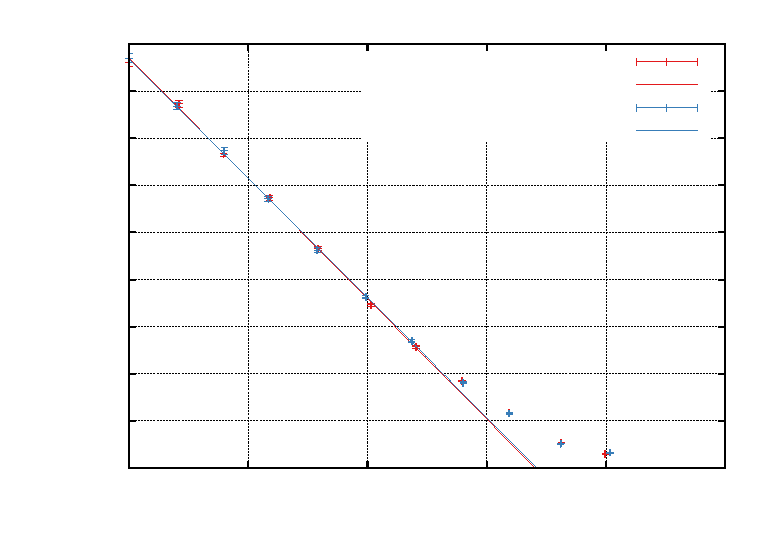
\includegraphics{./plots/photo/kennlinien_365nm}}%
    \gplfronttext
  \end{picture}%
\endgroup

	\caption{Linearisierung der Kennlinie bei einer Wellenlänge von $\lambda = \SI{365}{\nano\metre}$. }
	\label{fig:kennlinien_exemp_365nm}
\end{figure}
Um schließlich die Grenzspannung zu erhalten, wird an den linearen Teil der Kurve eine Gerade mithilfe eines Least-Squares-Verfahrens (\texttt{Gnuplot}) angepasst.
Die restlichen Linearisierungen wurden im Anhang \ref{app:kennlinien} zusammengetragen und die Ergebnisse der Anpassung in Tabelle \ref{tab:photoeffekt_fit_results} zusammengefasst.
\begin{table}[h]
	\centering
	\begin{tabular}{SSSSSSSS}
	\toprule
	{$\frac{\lambda}{\si{\nano\metre}}$} & {$\frac{m}{\si{\nano\ampere\tothe{1/2}\per\volt}}$} & {$\frac{\Delta m}{\si{\nano\ampere\tothe{1/2}\per\volt}}$} & {$\frac{b}{\si{\nano\ampere\tothe{1/2}}}$} & {$\frac{\Delta b}{\si{\nano\ampere\tothe{1/2}}}$} & {$\chi_\mathrm{d.o.f.}^2$} & {$\frac{U_G}{\si{\volt}}$} & {$\frac{\Delta U_G}{\si{\volt}}$} \\
	\midrule
	365 & -2.557 & 0.026 & 4.353 & 0.026 & 1.10 & 1.702 & 0.020 \\
	 & -2.539 & 0.023 & 4.345 & 0.021 & 0.75 & 1.711 & 0.017 \\
	 \midrule
	405 & -1.959 & 0.033 & 2.777 & 0.028 & 3.57 & 1.418 & 0.028 \\
	 & -1.957 & 0.024 & 2.772 & 0.02  & 1.81 & 1.416 & 0.020 \\
	 \midrule
	436 & -3.000 & 0.032 & 3.655 & 0.023 & 1.71 & 1.218 & 0.015 \\
	 & -3.003 & 0.046 & 3.661 & 0.033 & 3.75 & 1.219 & 0.022 \\
	 \midrule
	546 & -4.542 & 0.012 & 3.203 & 0.005 & 0.05 & 0.705 & 0.003 \\
	 & -4.464 & 0.043 & 3.189 & 0.015 & 0.64 & 0.714 & 0.008 \\
	 \midrule
	578 & -3.771 & 0.036 & 2.230 & 0.011 & 0.89 & 0.591 & 0.006 \\
	 & -3.860 & 0.017 & 2.285 & 0.006 & 0.19 & 0.592 & 0.003 \\
	\bottomrule
\end{tabular}

	\caption{Ergebnisse der Anpassung einer Geraden $f(x) = m \cdot x + b$ an die linearisierten Kennlinien bei verschiedenen Wellenlängen}
	\label{tab:photoeffekt_fit_results}
\end{table}
Bisschen was zum Chiquadrat HIER!!!
Mit den Ergebnissen der Anpassung kann nun die Grenzspannung $U_0$ als Schnittpunkt der Geraden mit der $x$-Achse berechnet werden, sodass wir:
\begin{align*}
	U_0 &= -\frac{b}{m} \\
	\Delta U_0 &= \sqrt{\frac{\Delta b^2}{m^2} + \frac{b^2}{m^4}\cdot \Delta m^2}
\end{align*}
erhalten.
Auf diese Weise wird $U_0$ für jede der zehn Anpassungen berechnet und in Tabelle \ref{tab:photoeffekt_grenzspannungen} zusammengefasst.
\begin{table}[h]
	\centering
	\begin{tabular}{SSSSSSSS}
	\toprule
	{$\lambda$ / $\si{\nano\metre}$} & {$U_0$ / $\si{\volt}$} & {$\Delta U_0$ / $\si{\volt}$} \\
	\midrule
	\multirow{2}{*}{365} & 1.702 & 0.020 \\
	 & 1.711 & 0.017 \\
	 \midrule
	\multirow{2}{*}{405} & 1.418 & 0.028 \\
	 & 1.416 & 0.020 \\
	 \midrule
	\multirow{2}{*}{436} & 1.218 & 0.015 \\
	 & 1.219 & 0.022 \\
	 \midrule
	\multirow{2}{*}{546} & 0.705 & 0.003 \\
	 & 0.714 & 0.008 \\
	 \midrule
	\multirow{2}{*}{578} & 0.591 & 0.006 \\
	 & 0.592 & 0.003 \\
	\bottomrule
\end{tabular}

	\caption{Grenzspannungen}
	\label{tab:photoeffekt_grenzspannungen}
\end{table}

\subsubsection{Berechnung des Planckschen Wirkungsquantums}
Um das Plancksche Wirkungsquantum aus den gemessenen Grenzspannungen $U_0$ bei verschiedenen Wellenlängen $\lambda$ zu berechnen, wird die Energiebilanz (REFERENZ!) des Photons verwendet.
Dazu wird die Grenzspannung gegen die Frequenz des einfallenden Lichts aufgetragen, um eine Gerade mit der Steigung $h/e$ zu erhalten.
Zunächst wird der varianzgewichtete Mittelwert verwendet, um jeweils zwei Messungen zu der gleichen Wellenlänge zu mitteln.
Dieser ist gegeben durch:
\begin{align*}
\bar{x} = \frac{\sum_i \frac{x_i}{\sigma_i^2}}{\sum_i \frac{1}{\sigma_i^2}}\text{,}
\end{align*}
wobei der Fehler des Mittelwerts
\begin{align*}
\sigma_{\bar{x}} = \frac{1}{\sqrt{\sum_i \frac{1}{\sigma_i^2}}}
\end{align*}
beträgt.
Außerdem wird die zur Wellenlänge $\lambda$ zugehörige Frequenz $\nu$ (in Näherung) durch die Dispersionsrelation von elektromagnetischen Wellen im Vakuum berechnet:
\begin{align*}
	\nu = \frac{c}{\lambda}
\end{align*}
Nach Berechnung von Frequenz und mittlerer Grenzspannung ergeben sich die Werte aus Tabelle \ref{tab:photoeffekt_planck_fitdaten}.
\begin{table}[h]
	\centering
	\begin{tabular}{SSS}
	\toprule
	{$\nu$ / \si{\tera\hertz}} & {$U_0$ / \si{\volt}} & {$\Delta U_0$ / \si{\volt}} \\
	\midrule
	821.35 & 1.708 & 0.013 \\
	740.23 & 1.417 & 0.016 \\
	687.60 & 1.219 & 0.013 \\
	549.07 & 0.706 & 0.002 \\
	518.67 & 0.592 & 0.003 \\
	\bottomrule
\end{tabular}

	\caption{Linearisierung zur Bestimmung von h}
	\label{tab:photoeffekt_planck_fitdaten}
\end{table}
Anschließend werden diese Werte in einem $U_0$-$\nu$-Diagramm aufgetragen und eine Ausgleichsgerade nach dem Least-Squares-Verfahren berechnet.
Die Anpassung der Gerade ergibt:
\begin{align*}
	U_0 = m \cdot \nu + b
\end{align*}
mit den Anpassungsparametern:
\begin{align*}
	m &= \SI{0.00370 +- 0.00002}{\volt\per\tera\hertz} \\
	b &= \SI{-1.326 +- 0.008}{\volt}
\end{align*}
Die Güte dieser Anpassung ist gegeben durch das reduzierte Chi-Quadrat $\chi_\mathrm{red.}^2 = \num{0,15}$, welches eine gute Übereinstimmung der Datenpunkte mit der Anpassungshypothese nahelegt.
Die Datenpunkte und die angepasste Gerade wurden in Abbildung \ref{fig:lin_h} aufgetragen.
\begin{figure}[h]
	\centering
	% GNUPLOT: LaTeX picture with Postscript
\begingroup
  \makeatletter
  \providecommand\color[2][]{%
    \GenericError{(gnuplot) \space\space\space\@spaces}{%
      Package color not loaded in conjunction with
      terminal option `colourtext'%
    }{See the gnuplot documentation for explanation.%
    }{Either use 'blacktext' in gnuplot or load the package
      color.sty in LaTeX.}%
    \renewcommand\color[2][]{}%
  }%
  \providecommand\includegraphics[2][]{%
    \GenericError{(gnuplot) \space\space\space\@spaces}{%
      Package graphicx or graphics not loaded%
    }{See the gnuplot documentation for explanation.%
    }{The gnuplot epslatex terminal needs graphicx.sty or graphics.sty.}%
    \renewcommand\includegraphics[2][]{}%
  }%
  \providecommand\rotatebox[2]{#2}%
  \@ifundefined{ifGPcolor}{%
    \newif\ifGPcolor
    \GPcolortrue
  }{}%
  \@ifundefined{ifGPblacktext}{%
    \newif\ifGPblacktext
    \GPblacktexttrue
  }{}%
  % define a \g@addto@macro without @ in the name:
  \let\gplgaddtomacro\g@addto@macro
  % define empty templates for all commands taking text:
  \gdef\gplbacktext{}%
  \gdef\gplfronttext{}%
  \makeatother
  \ifGPblacktext
    % no textcolor at all
    \def\colorrgb#1{}%
    \def\colorgray#1{}%
  \else
    % gray or color?
    \ifGPcolor
      \def\colorrgb#1{\color[rgb]{#1}}%
      \def\colorgray#1{\color[gray]{#1}}%
      \expandafter\def\csname LTw\endcsname{\color{white}}%
      \expandafter\def\csname LTb\endcsname{\color{black}}%
      \expandafter\def\csname LTa\endcsname{\color{black}}%
      \expandafter\def\csname LT0\endcsname{\color[rgb]{1,0,0}}%
      \expandafter\def\csname LT1\endcsname{\color[rgb]{0,1,0}}%
      \expandafter\def\csname LT2\endcsname{\color[rgb]{0,0,1}}%
      \expandafter\def\csname LT3\endcsname{\color[rgb]{1,0,1}}%
      \expandafter\def\csname LT4\endcsname{\color[rgb]{0,1,1}}%
      \expandafter\def\csname LT5\endcsname{\color[rgb]{1,1,0}}%
      \expandafter\def\csname LT6\endcsname{\color[rgb]{0,0,0}}%
      \expandafter\def\csname LT7\endcsname{\color[rgb]{1,0.3,0}}%
      \expandafter\def\csname LT8\endcsname{\color[rgb]{0.5,0.5,0.5}}%
    \else
      % gray
      \def\colorrgb#1{\color{black}}%
      \def\colorgray#1{\color[gray]{#1}}%
      \expandafter\def\csname LTw\endcsname{\color{white}}%
      \expandafter\def\csname LTb\endcsname{\color{black}}%
      \expandafter\def\csname LTa\endcsname{\color{black}}%
      \expandafter\def\csname LT0\endcsname{\color{black}}%
      \expandafter\def\csname LT1\endcsname{\color{black}}%
      \expandafter\def\csname LT2\endcsname{\color{black}}%
      \expandafter\def\csname LT3\endcsname{\color{black}}%
      \expandafter\def\csname LT4\endcsname{\color{black}}%
      \expandafter\def\csname LT5\endcsname{\color{black}}%
      \expandafter\def\csname LT6\endcsname{\color{black}}%
      \expandafter\def\csname LT7\endcsname{\color{black}}%
      \expandafter\def\csname LT8\endcsname{\color{black}}%
    \fi
  \fi
  \setlength{\unitlength}{0.0500bp}%
  \begin{picture}(7200.00,5040.00)%
    \gplgaddtomacro\gplbacktext{%
      \csname LTb\endcsname%
      \put(946,704){\makebox(0,0)[r]{\strut{} 0.4}}%
      \csname LTb\endcsname%
      \put(946,1213){\makebox(0,0)[r]{\strut{} 0.6}}%
      \csname LTb\endcsname%
      \put(946,1722){\makebox(0,0)[r]{\strut{} 0.8}}%
      \csname LTb\endcsname%
      \put(946,2231){\makebox(0,0)[r]{\strut{} 1}}%
      \csname LTb\endcsname%
      \put(946,2740){\makebox(0,0)[r]{\strut{} 1.2}}%
      \csname LTb\endcsname%
      \put(946,3248){\makebox(0,0)[r]{\strut{} 1.4}}%
      \csname LTb\endcsname%
      \put(946,3757){\makebox(0,0)[r]{\strut{} 1.6}}%
      \csname LTb\endcsname%
      \put(946,4266){\makebox(0,0)[r]{\strut{} 1.8}}%
      \csname LTb\endcsname%
      \put(946,4775){\makebox(0,0)[r]{\strut{} 2}}%
      \csname LTb\endcsname%
      \put(1078,484){\makebox(0,0){\strut{} 500}}%
      \csname LTb\endcsname%
      \put(1896,484){\makebox(0,0){\strut{} 550}}%
      \csname LTb\endcsname%
      \put(2714,484){\makebox(0,0){\strut{} 600}}%
      \csname LTb\endcsname%
      \put(3532,484){\makebox(0,0){\strut{} 650}}%
      \csname LTb\endcsname%
      \put(4349,484){\makebox(0,0){\strut{} 700}}%
      \csname LTb\endcsname%
      \put(5167,484){\makebox(0,0){\strut{} 750}}%
      \csname LTb\endcsname%
      \put(5985,484){\makebox(0,0){\strut{} 800}}%
      \csname LTb\endcsname%
      \put(6803,484){\makebox(0,0){\strut{} 850}}%
      \put(176,2739){\rotatebox{-270}{\makebox(0,0){\strut{}$U_0 \, / \, \si{\volt}$}}}%
      \put(3940,154){\makebox(0,0){\strut{}$\nu \, / \, \si{\tera\hertz}$}}%
      \put(3940,4665){\makebox(0,0){\strut{}}}%
    }%
    \gplgaddtomacro\gplfronttext{%
      \csname LTb\endcsname%
      \put(5816,1097){\makebox(0,0)[r]{\strut{}Messung 1}}%
      \csname LTb\endcsname%
      \put(5816,877){\makebox(0,0)[r]{\strut{}Regressionsgerade 1}}%
    }%
    \gplbacktext
    \put(0,0){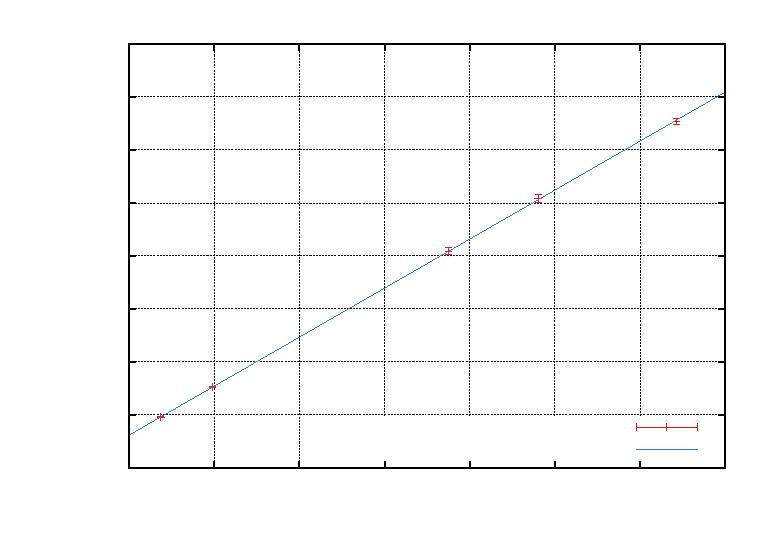
\includegraphics{./plots/planck_quantum_linearisierung}}%
    \gplfronttext
  \end{picture}%
\endgroup

	\caption{Linearisierung zur Bestimmung von $h$}
	\label{fig:lin_h}
\end{figure}
Zur Berechnung des Planckschen Wirkungsquantums wird die angepasste Gerade im Hinblick auf die Energiebilanz des Elektrons betrachtet.
Demnach ist die Steigung $m$ gegeben durch:
\begin{align*}
	m = \frac{h}{e}
\end{align*}
Das Wirkungsquantum wird durch Multiplikation der Steigung $m$ mit der Elementarladung\footnote{2010 CODATA recommended values\\\url{http://physics.nist.gov/cgi-bin/cuu/Value?e}\\Letzer Abruf: 6. Dezember 2014}:
\begin{align}
	e = \SI{1.602176565 +- 0.000000035e-19}{\coulomb}
\end{align}
berechnet, wobei der Einfluss des Fehlers der Elementarladung klein gegen den der Steigung ist und daher vernachlässigt wird.
Somit ergibt sich:
\begin{align*}
	h = \SI{5.93 +- 0.04}{\joule\second}
\end{align*}
(FEHLERDISKUSSION!)
Höchstwahrscheinlich systematischer Fehler bei Grenzspannungsbestimmung.

\subsubsection{Einfluss der Intensität auf die Kennlinien}
\begin{figure}[h]
	\centering
	% GNUPLOT: LaTeX picture with Postscript
\begingroup
  \makeatletter
  \providecommand\color[2][]{%
    \GenericError{(gnuplot) \space\space\space\@spaces}{%
      Package color not loaded in conjunction with
      terminal option `colourtext'%
    }{See the gnuplot documentation for explanation.%
    }{Either use 'blacktext' in gnuplot or load the package
      color.sty in LaTeX.}%
    \renewcommand\color[2][]{}%
  }%
  \providecommand\includegraphics[2][]{%
    \GenericError{(gnuplot) \space\space\space\@spaces}{%
      Package graphicx or graphics not loaded%
    }{See the gnuplot documentation for explanation.%
    }{The gnuplot epslatex terminal needs graphicx.sty or graphics.sty.}%
    \renewcommand\includegraphics[2][]{}%
  }%
  \providecommand\rotatebox[2]{#2}%
  \@ifundefined{ifGPcolor}{%
    \newif\ifGPcolor
    \GPcolortrue
  }{}%
  \@ifundefined{ifGPblacktext}{%
    \newif\ifGPblacktext
    \GPblacktexttrue
  }{}%
  % define a \g@addto@macro without @ in the name:
  \let\gplgaddtomacro\g@addto@macro
  % define empty templates for all commands taking text:
  \gdef\gplbacktext{}%
  \gdef\gplfronttext{}%
  \makeatother
  \ifGPblacktext
    % no textcolor at all
    \def\colorrgb#1{}%
    \def\colorgray#1{}%
  \else
    % gray or color?
    \ifGPcolor
      \def\colorrgb#1{\color[rgb]{#1}}%
      \def\colorgray#1{\color[gray]{#1}}%
      \expandafter\def\csname LTw\endcsname{\color{white}}%
      \expandafter\def\csname LTb\endcsname{\color{black}}%
      \expandafter\def\csname LTa\endcsname{\color{black}}%
      \expandafter\def\csname LT0\endcsname{\color[rgb]{1,0,0}}%
      \expandafter\def\csname LT1\endcsname{\color[rgb]{0,1,0}}%
      \expandafter\def\csname LT2\endcsname{\color[rgb]{0,0,1}}%
      \expandafter\def\csname LT3\endcsname{\color[rgb]{1,0,1}}%
      \expandafter\def\csname LT4\endcsname{\color[rgb]{0,1,1}}%
      \expandafter\def\csname LT5\endcsname{\color[rgb]{1,1,0}}%
      \expandafter\def\csname LT6\endcsname{\color[rgb]{0,0,0}}%
      \expandafter\def\csname LT7\endcsname{\color[rgb]{1,0.3,0}}%
      \expandafter\def\csname LT8\endcsname{\color[rgb]{0.5,0.5,0.5}}%
    \else
      % gray
      \def\colorrgb#1{\color{black}}%
      \def\colorgray#1{\color[gray]{#1}}%
      \expandafter\def\csname LTw\endcsname{\color{white}}%
      \expandafter\def\csname LTb\endcsname{\color{black}}%
      \expandafter\def\csname LTa\endcsname{\color{black}}%
      \expandafter\def\csname LT0\endcsname{\color{black}}%
      \expandafter\def\csname LT1\endcsname{\color{black}}%
      \expandafter\def\csname LT2\endcsname{\color{black}}%
      \expandafter\def\csname LT3\endcsname{\color{black}}%
      \expandafter\def\csname LT4\endcsname{\color{black}}%
      \expandafter\def\csname LT5\endcsname{\color{black}}%
      \expandafter\def\csname LT6\endcsname{\color{black}}%
      \expandafter\def\csname LT7\endcsname{\color{black}}%
      \expandafter\def\csname LT8\endcsname{\color{black}}%
    \fi
  \fi
  \setlength{\unitlength}{0.0500bp}%
  \begin{picture}(6480.00,4320.00)%
    \gplgaddtomacro\gplbacktext{%
      \csname LTb\endcsname%
      \put(814,820){\makebox(0,0)[r]{\strut{} 0}}%
      \csname LTb\endcsname%
      \put(814,1467){\makebox(0,0)[r]{\strut{} 5}}%
      \csname LTb\endcsname%
      \put(814,2114){\makebox(0,0)[r]{\strut{} 10}}%
      \csname LTb\endcsname%
      \put(814,2761){\makebox(0,0)[r]{\strut{} 15}}%
      \csname LTb\endcsname%
      \put(814,3408){\makebox(0,0)[r]{\strut{} 20}}%
      \csname LTb\endcsname%
      \put(814,4055){\makebox(0,0)[r]{\strut{} 25}}%
      \csname LTb\endcsname%
      \put(1068,484){\makebox(0,0){\strut{} 0}}%
      \csname LTb\endcsname%
      \put(2291,484){\makebox(0,0){\strut{} 0,5}}%
      \csname LTb\endcsname%
      \put(3515,484){\makebox(0,0){\strut{} 1}}%
      \csname LTb\endcsname%
      \put(4738,484){\makebox(0,0){\strut{} 1,5}}%
      \csname LTb\endcsname%
      \put(5961,484){\makebox(0,0){\strut{} 2}}%
      \put(176,2379){\rotatebox{-270}{\makebox(0,0){\strut{}$I-I_0 \, / \, \si{\nano\ampere}$}}}%
      \put(3514,154){\makebox(0,0){\strut{}$U \, / \, \si{\volt}$}}%
      \put(3514,3945){\makebox(0,0){\strut{}}}%
    }%
    \gplgaddtomacro\gplfronttext{%
      \csname LTb\endcsname%
      \put(5096,3882){\makebox(0,0)[r]{\strut{}Messung 1}}%
      \csname LTb\endcsname%
      \put(5096,3662){\makebox(0,0)[r]{\strut{}Messung 2}}%
    }%
    \gplbacktext
    \put(0,0){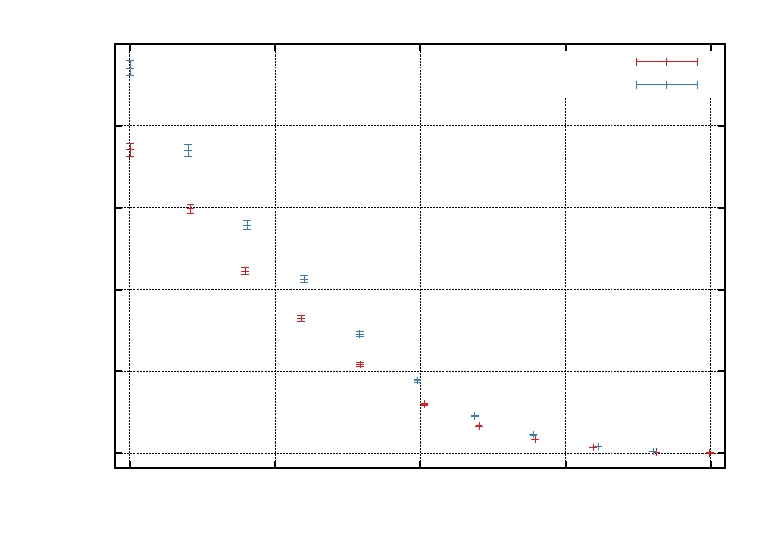
\includegraphics{./plots/kennlinie_intensitaet}}%
    \gplfronttext
  \end{picture}%
\endgroup

	\caption{Intensitätsvergleich der Kennlinien $\lambda = \SI{365}{\nano\metre}$}
	\label{fig:kennlinie_intensitaet}
\end{figure}
Bei der Durchführung wurde die Kennlinie der Photozelle bei der Wellenlänge $\lambda = \SI{365}{\nano\metre}$ jeweils bei zwei unterschiedlichen Intensitäten gemessen.
In Abbildung \ref{fig:kennlinie_intensitaet} wurden beide Kennlinien aufgetragen und im Folgenden soll deren Charakteristika diskutiert werden.
\begin{itemize}
	\item Zunächst signifikante Abweichung, mit steigender Spannung sinkt die Differenz der beiden Kennlinien.
	\item Klar zu erkennen -- Gleiche Grenzfrequenz! -- logisch da Elektronenenergie unabhängig von Intensität
\end{itemize}


\section{Balmer-Serie}

\subsection{Durchführung}

\subsubsection{Aufbau und Justage}
Wir setzen $\omega_\mathrm{B}$ konstant auf \SI{150}{\degree}.

\subsubsection{Bestimmung der Gitterkonstanten}
\begin{table}[h]
	\centering
	\begin{tabular}{SSS}
	\toprule
	{$\lambda$ / \si{\nano\metre}} & {$\omega_\mathrm{G}$ / \si{\degree}} & {$d$ / \si{\milli\metre}}\\
	\midrule
	404.656 & 46.0 & 2.10  \\
	407.783 & 46.0 & 0.00  \\
	410.805 & 46.0 & -2.10 \\
	\midrule
	433.922 & 48.5 & 1.30  \\
	434.749 & 48.5 & 0.70  \\
	435.833 & 48.5 & 0.00  \\
	\midrule
	491.607 & 53.5 & 0.00  \\
	\midrule
	546.074 & 58.5 & 0.00  \\
	\midrule
	576.960 & 62.0 & 1.70  \\
	579.066 & 62.0 & 0.00  \\
	\midrule
	623.440 & 67.0 & 0.00  \\
	\midrule
	671.643 & 72.5 & 0.00 \\
	\bottomrule
\end{tabular}

	\caption{Ergebnisse der $\Delta \omega_\mathrm{G} = \SI{0.5}{\degree}$ und $\Delta d = \SI{0.05}{\milli\metre}$}
	\label{tab:gitterkonstante_messdaten}
\end{table}
(Erklären warum wir die \SI{690}{\nano\metre} Linie nicht gemessen haben)

\subsubsection{Messung der Balmer-Linien mit einem Okular}

\subsubsection{Messung der Balmer-Linien mit einer CCD-Kamera}


\subsection{Auswertung}

\subsubsection{Bestimmung der Gitterkonstanten}
\begin{figure}[h]
	\centering
	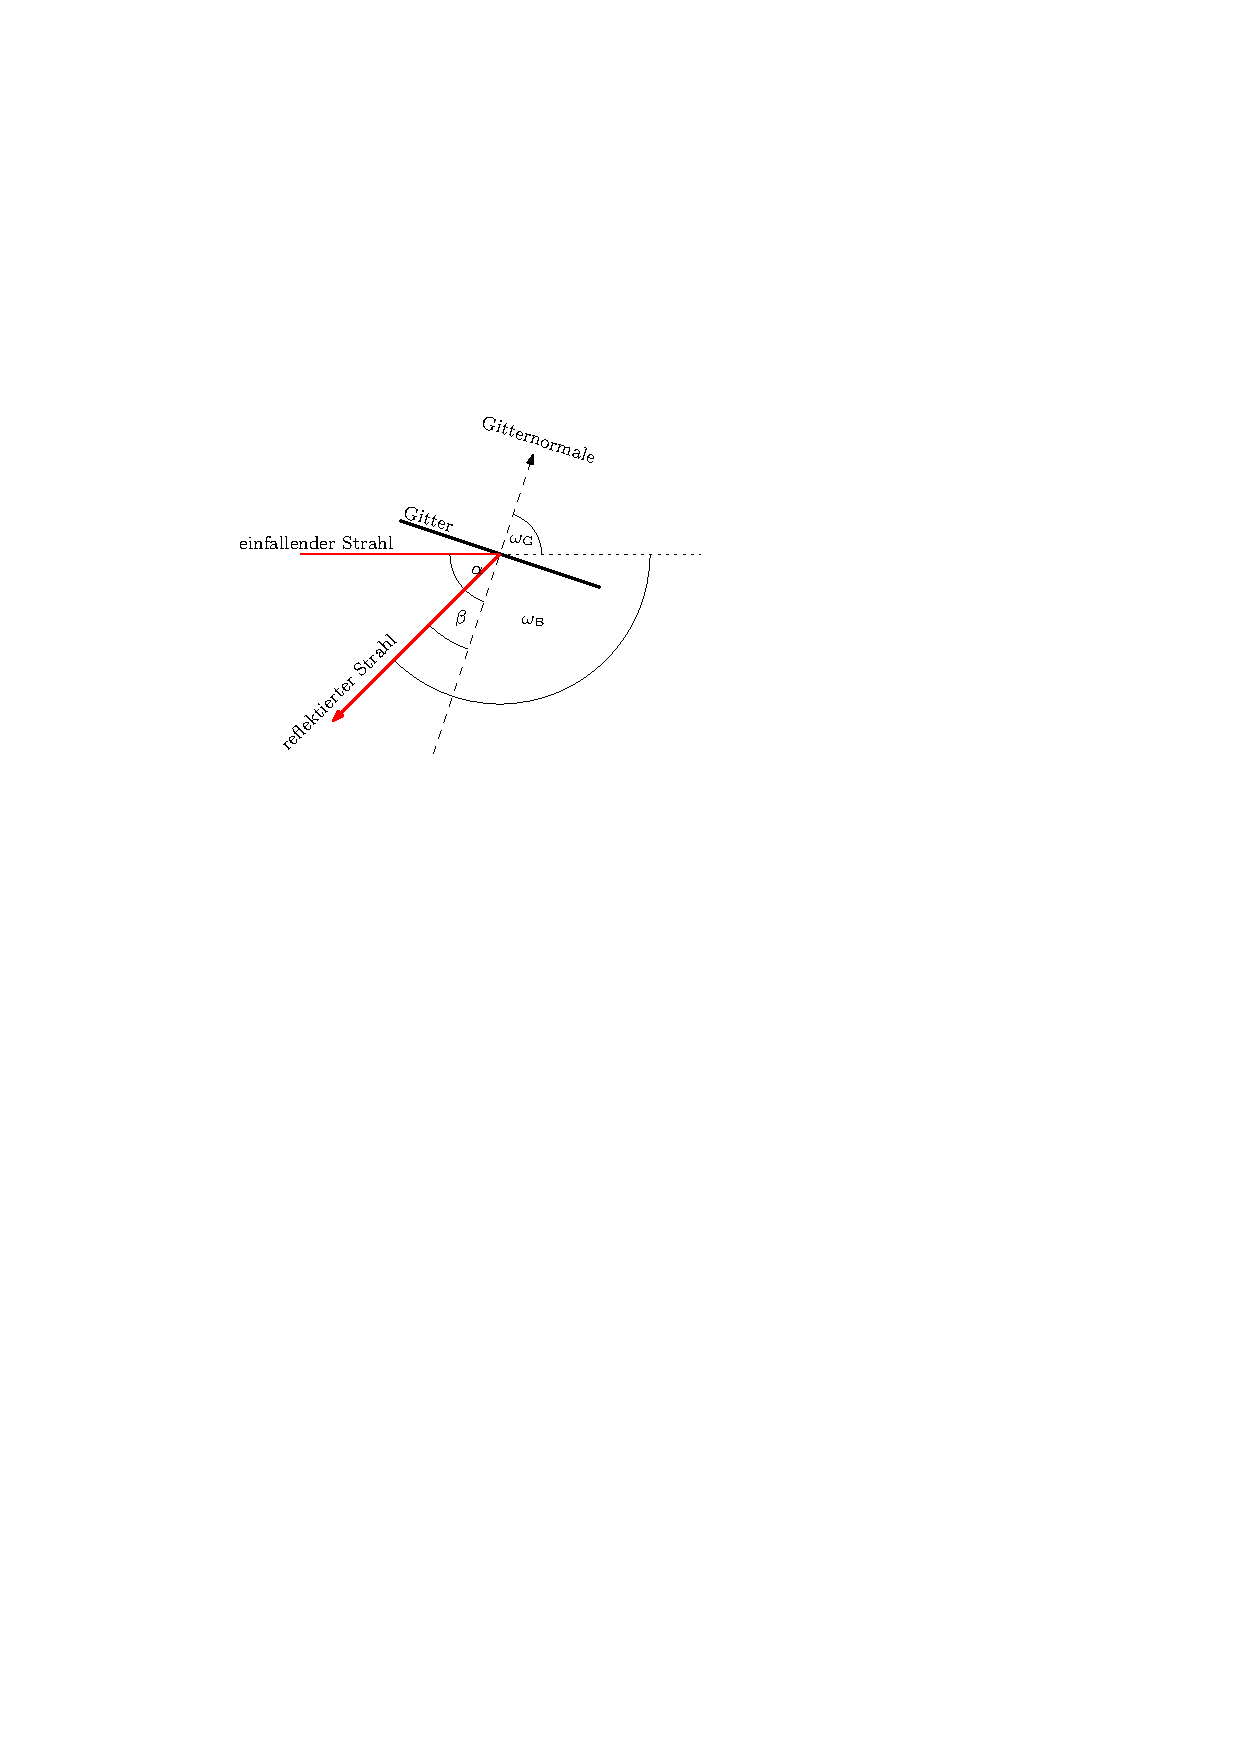
\includegraphics[width=0.65\textwidth]{./figures/winkelverhaeltniss.pdf}
	\caption{Winkelverhältnis zwischen Gitter und optischer Bank}
	\label{fig:winkelverhaeltnis}
\end{figure}
Aus Abbildung \ref{fig:winkelverhaeltnis} folgt der Zusammenhang zwischen gemessenen Winkeln und Ein-/Ausfallswinkel des Strahls auf das Gitter: 
\begin{align*}
	\alpha &= \omega_\text{G} \\
	\beta &= \omega_\text{G} + \omega_\text{B} - \SI{180}{\degree}
	\label{eq:reflexionswinkel}
\end{align*}
Korrektur des Ausfallswinkels aufgrund der Messung von $d$ mit dem Objektiv:
\begin{align*}
\Delta \beta = -\frac{d}{f} \text{ in KWN}
\end{align*}
$f$ Brennweite des Fernrohrobjektivs ($\SI{300}{\milli\metre}$).
So folgt der tatsächliche Ausfallswinkel gemäß:
\begin{align*}
	\beta^\prime = \beta + \Delta \beta
\end{align*}
Zur Bestimmung der Gitterkonstanten tragen wir $\sin(\alpha) + \sin(\beta)$ gegen $\lambda$ auf, um mit der Gittergleichung
\begin{align*}
	\sin(\alpha) + \sin(\beta) = \frac{1}{g} \cdot \lambda
\end{align*}
zu erhalten.
Wir wählen diese Form der Gleichung, da bei einer Anpassung mit üblichen Least-Squares-Verfahren nur Fehler in $y$-Richtung beachtet werden.
Da der Fehler der Wellenlänge $\lambda$ gegen den der Sinus-Summe vernachlässigbar ist, wurde diese Form gewählt (\#machmalrichtig).
Wir erhalten für die Anpassung:
\begin{align}
	\sin(\alpha) + \sin(\beta) = \SI{2439.6 +- 2.1}{\per\milli\metre} \cdot \lambda \text{,}
\end{align}
was einer Gitterkonstanten in reziproken Einheiten von:
\begin{align*}
	\frac{1}{g} = (\num{2439.6 +- 2.1}) \, \frac{\mathrm{Linien}}{\si{\milli\metre}}
\end{align*}
entspricht.
Nach Kehrwertbildung ergibt sich:
\begin{align*}
	g = \SI{409.90 +- 0.36}{\nano\metre} \text{.}
\end{align*}


\subsection{Isotopieaufspaltung mit Okular}

Geradenfit:
\begin{align*}
	\frac{1}{\lambda} = R \cdot \left( \frac{1}{4} - \frac{1}{n^2} \right) \quad \text{mit} \quad R = \SI{11.0163 +- 0.02154}{\per\micro\metre}
\end{align*}
\begin{align*}
	\chi_\mathrm{red.}^2 = \num{0.263}
\end{align*}


\subsubsection{Durchführung}
\label{sec:balmer_okular}

\subsection{Isotopieaufspaltung mit CCD Kamera}

\subsubsection{Durchführung}

Wir nutzen den Versuchsaufbau wie in \ref{sec:balmer_okular} beschrieben, ersetzen das Okular jedoch durch eine CCD Kamera, die wir mit dem Computer verbinden.
Im Programm VideoCom wird die Brennweite der auf die CCD-Zeile abbildenden Linse (\SI{300}{\milli\meter}) eingetragen, so dass jedem der 2048 ein Winkel zugeordnet werden kann, den wir im folgenden mit $\alpha$ bezeichnen.
Um die Linien aufzufinden nutzen wir das Okular auf einem zusätzlichen Reiter (um die vertikale Ausrichtung bei jedem Durchgang nicht anpassen zu müssen) und drehen das Gitter entsprechend, bis die Linie möglichst zentral liegt.
Dann setzen wir den Reiter mit der Kamera anstelle des Okulars auf die optische Bank und betrachten das Intensitätsprofil auf dem Bildschirm, um die Abbildungslinse so zu verschieben, bis wir scharf auf die Kamera abbilden.
Wir vergrößern nun den Bildausschnitt, um den Bereich der Linie besser betrachten zu können und verändern die Spaltbreite so, dass wir eine möglichst hohe Intensität und gleichzeitig eine gute Aufspaltung messen.
Da dies nicht immer eindeutig gelang haben wir zu jeder Linie mehrere Messungen durchgeführt und zur Auswertung jeweils die Messung gewählt, bei der die Aufspaltung gut zu erkennen war.
Wegen der teilweise hohen Schwankungen der Intensität haben wir die Messwerte im Programm über eine gewisse Zeit mitteln lassen, bis mit dem Auge beinahe keine Schwankungen mehr zu erkennen waren.

\subsubsection{Auswertung}

Wir wählen wie bereits erwähnt die jeweils beste Messung aus den vorliegenden Daten aus und stellen die Aufspaltung grafisch dar.
Dabei passen wir mit \texttt{gnuplot} (least-squares-fit) zwei Gaußfunktionen an die Maxima mit folgender Fithypothese an:
\begin{align}
f(x)&=\mathcal{G}_1(x)+\mathcal{G}_2(x) + d\qquad\text{mit}\\
\mathcal{G}_i(x)&=A\,\exp\left[-\frac{1}{2}\left(\frac{x-S_i}{\sigma_i}\right)^2\right]
\end{align}
Diese sind zusammen mit den Messdaten in den Abbildungen \ref{fig:aufspaltung_rot} bis  \ref{fig:aufspaltung_violett} dargestellt.
Die Isotopieaufspaltung der violetten Balmer-Linie ist dabei so klein, dass wir sie nicht messen konnten.
Der Vollständigkeit halber haben wir die Messwerte und eine daran angepasste Gaußkurve in dieses Protokoll aufgenommen, eine Auswertung ist damit jedoch nicht möglich.\\
\\
Für den Intensitätsfehler haben wir mit Berücksichtigung der Mittelung der Messwerte über einen Zeitraum (die genommenen Daten unterliegen deswegen sehr kleinen Schwankungen) \SI{0.2}{\percent} für die Daten zur roten und türkisen Linie angenommen.
Für die blaue Linie haben wir aufgrund der geringen Intensität sehr lange im Programm VideoCom mitteln lassen und wählen deswegen \SI{0.1}{\percent} als Fehler für die Intensität.
Den Fehler des Winkels schätzen wir zu \SI{0.0015}{\degree} ab; dies folgt aus der Überlegung, dass wir einen Winkelbereich von ca. \SI{5.5}{\degree} auf \num{2048} Pixeln messen.
\begin{figure}[h]
\centering
% GNUPLOT: LaTeX picture with Postscript
\begingroup
  \makeatletter
  \providecommand\color[2][]{%
    \GenericError{(gnuplot) \space\space\space\@spaces}{%
      Package color not loaded in conjunction with
      terminal option `colourtext'%
    }{See the gnuplot documentation for explanation.%
    }{Either use 'blacktext' in gnuplot or load the package
      color.sty in LaTeX.}%
    \renewcommand\color[2][]{}%
  }%
  \providecommand\includegraphics[2][]{%
    \GenericError{(gnuplot) \space\space\space\@spaces}{%
      Package graphicx or graphics not loaded%
    }{See the gnuplot documentation for explanation.%
    }{The gnuplot epslatex terminal needs graphicx.sty or graphics.sty.}%
    \renewcommand\includegraphics[2][]{}%
  }%
  \providecommand\rotatebox[2]{#2}%
  \@ifundefined{ifGPcolor}{%
    \newif\ifGPcolor
    \GPcolortrue
  }{}%
  \@ifundefined{ifGPblacktext}{%
    \newif\ifGPblacktext
    \GPblacktexttrue
  }{}%
  % define a \g@addto@macro without @ in the name:
  \let\gplgaddtomacro\g@addto@macro
  % define empty templates for all commands taking text:
  \gdef\gplbacktext{}%
  \gdef\gplfronttext{}%
  \makeatother
  \ifGPblacktext
    % no textcolor at all
    \def\colorrgb#1{}%
    \def\colorgray#1{}%
  \else
    % gray or color?
    \ifGPcolor
      \def\colorrgb#1{\color[rgb]{#1}}%
      \def\colorgray#1{\color[gray]{#1}}%
      \expandafter\def\csname LTw\endcsname{\color{white}}%
      \expandafter\def\csname LTb\endcsname{\color{black}}%
      \expandafter\def\csname LTa\endcsname{\color{black}}%
      \expandafter\def\csname LT0\endcsname{\color[rgb]{1,0,0}}%
      \expandafter\def\csname LT1\endcsname{\color[rgb]{0,1,0}}%
      \expandafter\def\csname LT2\endcsname{\color[rgb]{0,0,1}}%
      \expandafter\def\csname LT3\endcsname{\color[rgb]{1,0,1}}%
      \expandafter\def\csname LT4\endcsname{\color[rgb]{0,1,1}}%
      \expandafter\def\csname LT5\endcsname{\color[rgb]{1,1,0}}%
      \expandafter\def\csname LT6\endcsname{\color[rgb]{0,0,0}}%
      \expandafter\def\csname LT7\endcsname{\color[rgb]{1,0.3,0}}%
      \expandafter\def\csname LT8\endcsname{\color[rgb]{0.5,0.5,0.5}}%
    \else
      % gray
      \def\colorrgb#1{\color{black}}%
      \def\colorgray#1{\color[gray]{#1}}%
      \expandafter\def\csname LTw\endcsname{\color{white}}%
      \expandafter\def\csname LTb\endcsname{\color{black}}%
      \expandafter\def\csname LTa\endcsname{\color{black}}%
      \expandafter\def\csname LT0\endcsname{\color{black}}%
      \expandafter\def\csname LT1\endcsname{\color{black}}%
      \expandafter\def\csname LT2\endcsname{\color{black}}%
      \expandafter\def\csname LT3\endcsname{\color{black}}%
      \expandafter\def\csname LT4\endcsname{\color{black}}%
      \expandafter\def\csname LT5\endcsname{\color{black}}%
      \expandafter\def\csname LT6\endcsname{\color{black}}%
      \expandafter\def\csname LT7\endcsname{\color{black}}%
      \expandafter\def\csname LT8\endcsname{\color{black}}%
    \fi
  \fi
  \setlength{\unitlength}{0.0500bp}%
  \begin{picture}(7486.00,5040.00)%
    \gplgaddtomacro\gplbacktext{%
      \csname LTb\endcsname%
      \put(814,704){\makebox(0,0)[r]{\strut{} 0}}%
      \csname LTb\endcsname%
      \put(814,1286){\makebox(0,0)[r]{\strut{} 5}}%
      \csname LTb\endcsname%
      \put(814,1867){\makebox(0,0)[r]{\strut{} 10}}%
      \csname LTb\endcsname%
      \put(814,2449){\makebox(0,0)[r]{\strut{} 15}}%
      \csname LTb\endcsname%
      \put(814,3030){\makebox(0,0)[r]{\strut{} 20}}%
      \csname LTb\endcsname%
      \put(814,3612){\makebox(0,0)[r]{\strut{} 25}}%
      \csname LTb\endcsname%
      \put(814,4193){\makebox(0,0)[r]{\strut{} 30}}%
      \csname LTb\endcsname%
      \put(814,4775){\makebox(0,0)[r]{\strut{} 35}}%
      \csname LTb\endcsname%
      \put(946,484){\makebox(0,0){\strut{} 0.11}}%
      \csname LTb\endcsname%
      \put(1714,484){\makebox(0,0){\strut{} 0.12}}%
      \csname LTb\endcsname%
      \put(2482,484){\makebox(0,0){\strut{} 0.13}}%
      \csname LTb\endcsname%
      \put(3250,484){\makebox(0,0){\strut{} 0.14}}%
      \csname LTb\endcsname%
      \put(4018,484){\makebox(0,0){\strut{} 0.15}}%
      \csname LTb\endcsname%
      \put(4785,484){\makebox(0,0){\strut{} 0.16}}%
      \csname LTb\endcsname%
      \put(5553,484){\makebox(0,0){\strut{} 0.17}}%
      \csname LTb\endcsname%
      \put(6321,484){\makebox(0,0){\strut{} 0.18}}%
      \csname LTb\endcsname%
      \put(7089,484){\makebox(0,0){\strut{} 0.19}}%
      \put(176,2739){\rotatebox{-270}{\makebox(0,0){\strut{}Intensität $I$ / \si{\percent}}}}%
      \put(4017,154){\makebox(0,0){\strut{}Winkel $\alpha$ / \si{\degree}}}%
      \put(4017,4665){\makebox(0,0){\strut{}}}%
    }%
    \gplgaddtomacro\gplfronttext{%
      \csname LTb\endcsname%
      \put(6102,4602){\makebox(0,0)[r]{\strut{}Messwerte}}%
      \csname LTb\endcsname%
      \put(6102,4382){\makebox(0,0)[r]{\strut{}$\Sigma$}}%
      \csname LTb\endcsname%
      \put(6102,4162){\makebox(0,0)[r]{\strut{}$\mathcal{G}_1$}}%
      \csname LTb\endcsname%
      \put(6102,3942){\makebox(0,0)[r]{\strut{}$\mathcal{G}_2$}}%
      \csname LTb\endcsname%
      \put(6102,3722){\makebox(0,0)[r]{\strut{}$d$}}%
    }%
    \gplbacktext
    \put(0,0){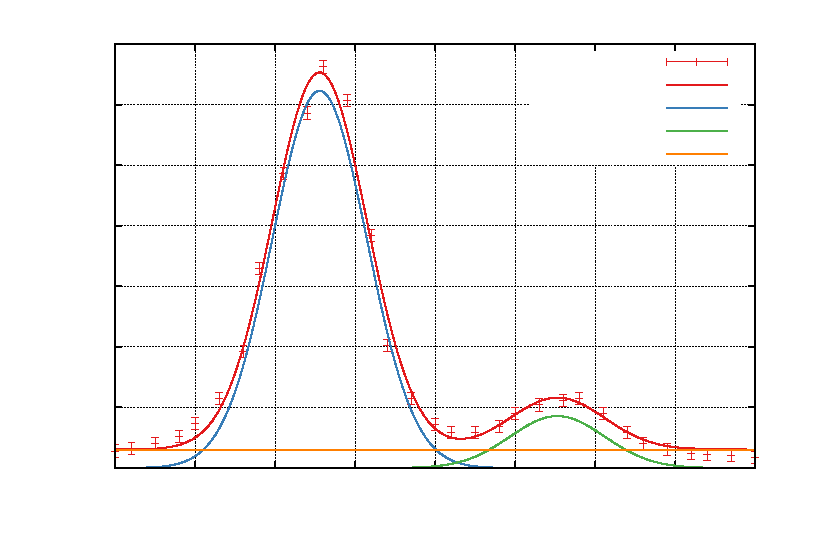
\includegraphics{./plots/aufspaltung/rot2}}%
    \gplfronttext
  \end{picture}%
\endgroup

\caption{Isotopieaufspaltung der roten Balmer-Linien von Wasserstoff und Deuterium}
\label{fig:aufspaltung_rot}
\end{figure}
\begin{figure}[h]
\centering
% GNUPLOT: LaTeX picture with Postscript
\begingroup
  \makeatletter
  \providecommand\color[2][]{%
    \GenericError{(gnuplot) \space\space\space\@spaces}{%
      Package color not loaded in conjunction with
      terminal option `colourtext'%
    }{See the gnuplot documentation for explanation.%
    }{Either use 'blacktext' in gnuplot or load the package
      color.sty in LaTeX.}%
    \renewcommand\color[2][]{}%
  }%
  \providecommand\includegraphics[2][]{%
    \GenericError{(gnuplot) \space\space\space\@spaces}{%
      Package graphicx or graphics not loaded%
    }{See the gnuplot documentation for explanation.%
    }{The gnuplot epslatex terminal needs graphicx.sty or graphics.sty.}%
    \renewcommand\includegraphics[2][]{}%
  }%
  \providecommand\rotatebox[2]{#2}%
  \@ifundefined{ifGPcolor}{%
    \newif\ifGPcolor
    \GPcolortrue
  }{}%
  \@ifundefined{ifGPblacktext}{%
    \newif\ifGPblacktext
    \GPblacktexttrue
  }{}%
  % define a \g@addto@macro without @ in the name:
  \let\gplgaddtomacro\g@addto@macro
  % define empty templates for all commands taking text:
  \gdef\gplbacktext{}%
  \gdef\gplfronttext{}%
  \makeatother
  \ifGPblacktext
    % no textcolor at all
    \def\colorrgb#1{}%
    \def\colorgray#1{}%
  \else
    % gray or color?
    \ifGPcolor
      \def\colorrgb#1{\color[rgb]{#1}}%
      \def\colorgray#1{\color[gray]{#1}}%
      \expandafter\def\csname LTw\endcsname{\color{white}}%
      \expandafter\def\csname LTb\endcsname{\color{black}}%
      \expandafter\def\csname LTa\endcsname{\color{black}}%
      \expandafter\def\csname LT0\endcsname{\color[rgb]{1,0,0}}%
      \expandafter\def\csname LT1\endcsname{\color[rgb]{0,1,0}}%
      \expandafter\def\csname LT2\endcsname{\color[rgb]{0,0,1}}%
      \expandafter\def\csname LT3\endcsname{\color[rgb]{1,0,1}}%
      \expandafter\def\csname LT4\endcsname{\color[rgb]{0,1,1}}%
      \expandafter\def\csname LT5\endcsname{\color[rgb]{1,1,0}}%
      \expandafter\def\csname LT6\endcsname{\color[rgb]{0,0,0}}%
      \expandafter\def\csname LT7\endcsname{\color[rgb]{1,0.3,0}}%
      \expandafter\def\csname LT8\endcsname{\color[rgb]{0.5,0.5,0.5}}%
    \else
      % gray
      \def\colorrgb#1{\color{black}}%
      \def\colorgray#1{\color[gray]{#1}}%
      \expandafter\def\csname LTw\endcsname{\color{white}}%
      \expandafter\def\csname LTb\endcsname{\color{black}}%
      \expandafter\def\csname LTa\endcsname{\color{black}}%
      \expandafter\def\csname LT0\endcsname{\color{black}}%
      \expandafter\def\csname LT1\endcsname{\color{black}}%
      \expandafter\def\csname LT2\endcsname{\color{black}}%
      \expandafter\def\csname LT3\endcsname{\color{black}}%
      \expandafter\def\csname LT4\endcsname{\color{black}}%
      \expandafter\def\csname LT5\endcsname{\color{black}}%
      \expandafter\def\csname LT6\endcsname{\color{black}}%
      \expandafter\def\csname LT7\endcsname{\color{black}}%
      \expandafter\def\csname LT8\endcsname{\color{black}}%
    \fi
  \fi
  \setlength{\unitlength}{0.0500bp}%
  \begin{picture}(7486.00,5040.00)%
    \gplgaddtomacro\gplbacktext{%
      \csname LTb\endcsname%
      \put(814,704){\makebox(0,0)[r]{\strut{} 0}}%
      \csname LTb\endcsname%
      \put(814,1383){\makebox(0,0)[r]{\strut{} 2}}%
      \csname LTb\endcsname%
      \put(814,2061){\makebox(0,0)[r]{\strut{} 4}}%
      \csname LTb\endcsname%
      \put(814,2740){\makebox(0,0)[r]{\strut{} 6}}%
      \csname LTb\endcsname%
      \put(814,3418){\makebox(0,0)[r]{\strut{} 8}}%
      \csname LTb\endcsname%
      \put(814,4097){\makebox(0,0)[r]{\strut{} 10}}%
      \csname LTb\endcsname%
      \put(814,4775){\makebox(0,0)[r]{\strut{} 12}}%
      \csname LTb\endcsname%
      \put(946,484){\makebox(0,0){\strut{} 0,06}}%
      \csname LTb\endcsname%
      \put(1629,484){\makebox(0,0){\strut{} 0,065}}%
      \csname LTb\endcsname%
      \put(2311,484){\makebox(0,0){\strut{} 0,07}}%
      \csname LTb\endcsname%
      \put(2994,484){\makebox(0,0){\strut{} 0,075}}%
      \csname LTb\endcsname%
      \put(3676,484){\makebox(0,0){\strut{} 0,08}}%
      \csname LTb\endcsname%
      \put(4359,484){\makebox(0,0){\strut{} 0,085}}%
      \csname LTb\endcsname%
      \put(5041,484){\makebox(0,0){\strut{} 0,09}}%
      \csname LTb\endcsname%
      \put(5724,484){\makebox(0,0){\strut{} 0,095}}%
      \csname LTb\endcsname%
      \put(6406,484){\makebox(0,0){\strut{} 0,1}}%
      \csname LTb\endcsname%
      \put(7089,484){\makebox(0,0){\strut{} 0,105}}%
      \put(176,2739){\rotatebox{-270}{\makebox(0,0){\strut{}Intensität $I$ / \si{\percent}}}}%
      \put(4017,154){\makebox(0,0){\strut{}Winkel $\alpha$ / \si{\degree}}}%
      \put(4017,4665){\makebox(0,0){\strut{}}}%
    }%
    \gplgaddtomacro\gplfronttext{%
      \csname LTb\endcsname%
      \put(6102,4602){\makebox(0,0)[r]{\strut{}Messwerte}}%
      \csname LTb\endcsname%
      \put(6102,4382){\makebox(0,0)[r]{\strut{}$\Sigma$}}%
      \csname LTb\endcsname%
      \put(6102,4162){\makebox(0,0)[r]{\strut{}$\mathcal{G}_1$}}%
      \csname LTb\endcsname%
      \put(6102,3942){\makebox(0,0)[r]{\strut{}$\mathcal{G}_2$}}%
      \csname LTb\endcsname%
      \put(6102,3722){\makebox(0,0)[r]{\strut{}$d$}}%
    }%
    \gplbacktext
    \put(0,0){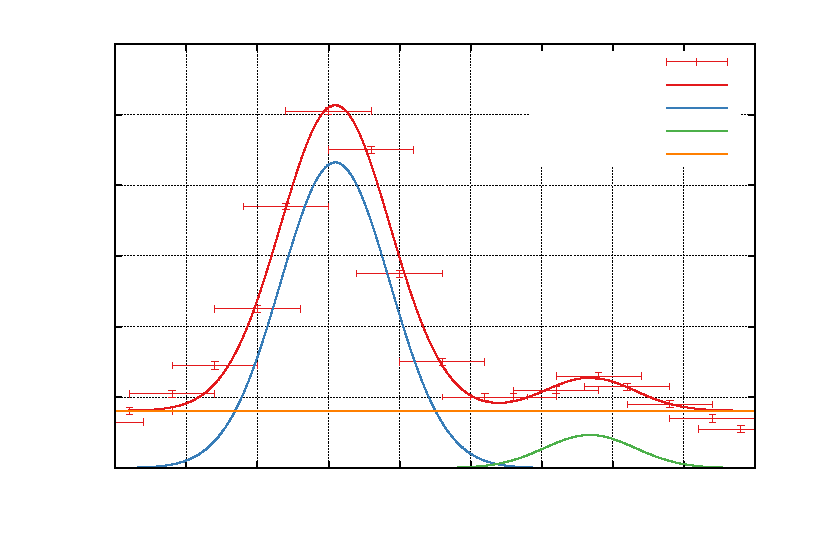
\includegraphics{./plots/aufspaltung/tuerkis1}}%
    \gplfronttext
  \end{picture}%
\endgroup

\caption{Isotopieaufspaltung der türkisen Balmer-Linien von Wasserstoff und Deuterium}
\label{fig:aufspaltung_tuerkis}
\end{figure}
\begin{figure}[h]
\centering
% GNUPLOT: LaTeX picture with Postscript
\begingroup
  \makeatletter
  \providecommand\color[2][]{%
    \GenericError{(gnuplot) \space\space\space\@spaces}{%
      Package color not loaded in conjunction with
      terminal option `colourtext'%
    }{See the gnuplot documentation for explanation.%
    }{Either use 'blacktext' in gnuplot or load the package
      color.sty in LaTeX.}%
    \renewcommand\color[2][]{}%
  }%
  \providecommand\includegraphics[2][]{%
    \GenericError{(gnuplot) \space\space\space\@spaces}{%
      Package graphicx or graphics not loaded%
    }{See the gnuplot documentation for explanation.%
    }{The gnuplot epslatex terminal needs graphicx.sty or graphics.sty.}%
    \renewcommand\includegraphics[2][]{}%
  }%
  \providecommand\rotatebox[2]{#2}%
  \@ifundefined{ifGPcolor}{%
    \newif\ifGPcolor
    \GPcolortrue
  }{}%
  \@ifundefined{ifGPblacktext}{%
    \newif\ifGPblacktext
    \GPblacktexttrue
  }{}%
  % define a \g@addto@macro without @ in the name:
  \let\gplgaddtomacro\g@addto@macro
  % define empty templates for all commands taking text:
  \gdef\gplbacktext{}%
  \gdef\gplfronttext{}%
  \makeatother
  \ifGPblacktext
    % no textcolor at all
    \def\colorrgb#1{}%
    \def\colorgray#1{}%
  \else
    % gray or color?
    \ifGPcolor
      \def\colorrgb#1{\color[rgb]{#1}}%
      \def\colorgray#1{\color[gray]{#1}}%
      \expandafter\def\csname LTw\endcsname{\color{white}}%
      \expandafter\def\csname LTb\endcsname{\color{black}}%
      \expandafter\def\csname LTa\endcsname{\color{black}}%
      \expandafter\def\csname LT0\endcsname{\color[rgb]{1,0,0}}%
      \expandafter\def\csname LT1\endcsname{\color[rgb]{0,1,0}}%
      \expandafter\def\csname LT2\endcsname{\color[rgb]{0,0,1}}%
      \expandafter\def\csname LT3\endcsname{\color[rgb]{1,0,1}}%
      \expandafter\def\csname LT4\endcsname{\color[rgb]{0,1,1}}%
      \expandafter\def\csname LT5\endcsname{\color[rgb]{1,1,0}}%
      \expandafter\def\csname LT6\endcsname{\color[rgb]{0,0,0}}%
      \expandafter\def\csname LT7\endcsname{\color[rgb]{1,0.3,0}}%
      \expandafter\def\csname LT8\endcsname{\color[rgb]{0.5,0.5,0.5}}%
    \else
      % gray
      \def\colorrgb#1{\color{black}}%
      \def\colorgray#1{\color[gray]{#1}}%
      \expandafter\def\csname LTw\endcsname{\color{white}}%
      \expandafter\def\csname LTb\endcsname{\color{black}}%
      \expandafter\def\csname LTa\endcsname{\color{black}}%
      \expandafter\def\csname LT0\endcsname{\color{black}}%
      \expandafter\def\csname LT1\endcsname{\color{black}}%
      \expandafter\def\csname LT2\endcsname{\color{black}}%
      \expandafter\def\csname LT3\endcsname{\color{black}}%
      \expandafter\def\csname LT4\endcsname{\color{black}}%
      \expandafter\def\csname LT5\endcsname{\color{black}}%
      \expandafter\def\csname LT6\endcsname{\color{black}}%
      \expandafter\def\csname LT7\endcsname{\color{black}}%
      \expandafter\def\csname LT8\endcsname{\color{black}}%
    \fi
  \fi
  \setlength{\unitlength}{0.0500bp}%
  \begin{picture}(7488.00,5040.00)%
    \gplgaddtomacro\gplbacktext{%
      \csname LTb\endcsname%
      \put(946,704){\makebox(0,0)[r]{\strut{} 0}}%
      \csname LTb\endcsname%
      \put(946,1286){\makebox(0,0)[r]{\strut{} 0,5}}%
      \csname LTb\endcsname%
      \put(946,1867){\makebox(0,0)[r]{\strut{} 1}}%
      \csname LTb\endcsname%
      \put(946,2449){\makebox(0,0)[r]{\strut{} 1,5}}%
      \csname LTb\endcsname%
      \put(946,3030){\makebox(0,0)[r]{\strut{} 2}}%
      \csname LTb\endcsname%
      \put(946,3612){\makebox(0,0)[r]{\strut{} 2,5}}%
      \csname LTb\endcsname%
      \put(946,4193){\makebox(0,0)[r]{\strut{} 3}}%
      \csname LTb\endcsname%
      \put(946,4775){\makebox(0,0)[r]{\strut{} 3,5}}%
      \csname LTb\endcsname%
      \put(1078,484){\makebox(0,0){\strut{}-0,03}}%
      \csname LTb\endcsname%
      \put(1746,484){\makebox(0,0){\strut{}-0,02}}%
      \csname LTb\endcsname%
      \put(2414,484){\makebox(0,0){\strut{}-0,01}}%
      \csname LTb\endcsname%
      \put(3082,484){\makebox(0,0){\strut{} 0}}%
      \csname LTb\endcsname%
      \put(3750,484){\makebox(0,0){\strut{} 0,01}}%
      \csname LTb\endcsname%
      \put(4419,484){\makebox(0,0){\strut{} 0,02}}%
      \csname LTb\endcsname%
      \put(5087,484){\makebox(0,0){\strut{} 0,03}}%
      \csname LTb\endcsname%
      \put(5755,484){\makebox(0,0){\strut{} 0,04}}%
      \csname LTb\endcsname%
      \put(6423,484){\makebox(0,0){\strut{} 0,05}}%
      \csname LTb\endcsname%
      \put(7091,484){\makebox(0,0){\strut{} 0,06}}%
      \put(176,2739){\rotatebox{-270}{\makebox(0,0){\strut{}Intensität $I$ / \si{\percent}}}}%
      \put(4084,154){\makebox(0,0){\strut{}Winkel $\delta$ / \si{\degree}}}%
      \put(4084,4665){\makebox(0,0){\strut{}}}%
    }%
    \gplgaddtomacro\gplfronttext{%
      \csname LTb\endcsname%
      \put(6104,4602){\makebox(0,0)[r]{\strut{}Messwerte}}%
      \csname LTb\endcsname%
      \put(6104,4382){\makebox(0,0)[r]{\strut{}$\Sigma$}}%
      \csname LTb\endcsname%
      \put(6104,4162){\makebox(0,0)[r]{\strut{}$\mathcal{G}_1$}}%
      \csname LTb\endcsname%
      \put(6104,3942){\makebox(0,0)[r]{\strut{}$\mathcal{G}_2$}}%
      \csname LTb\endcsname%
      \put(6104,3722){\makebox(0,0)[r]{\strut{}$d$}}%
    }%
    \gplbacktext
    \put(0,0){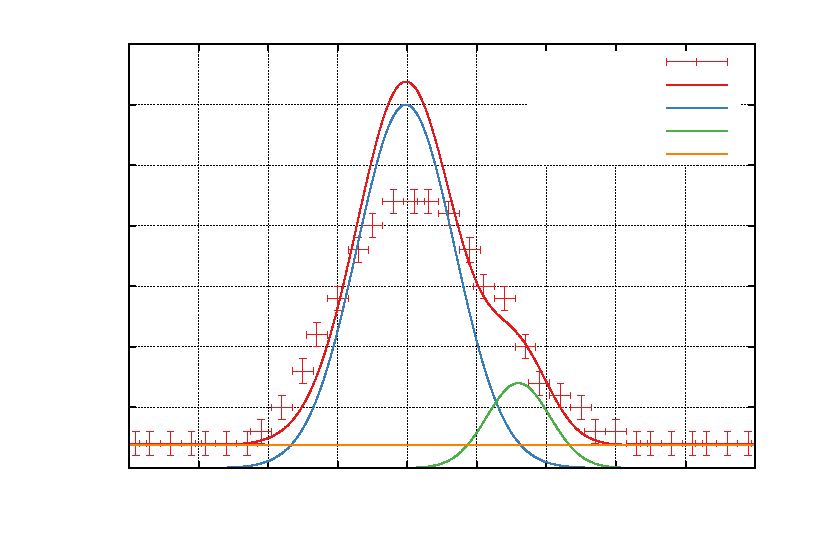
\includegraphics{./plots/aufspaltung/blau1}}%
    \gplfronttext
  \end{picture}%
\endgroup

\caption{Isotopieaufspaltung der blauen Balmer-Linien von Wasserstoff und Deuterium}
\label{fig:aufspaltung_blau}
\end{figure}
\begin{figure}[h]
\centering
% GNUPLOT: LaTeX picture with Postscript
\begingroup
  \makeatletter
  \providecommand\color[2][]{%
    \GenericError{(gnuplot) \space\space\space\@spaces}{%
      Package color not loaded in conjunction with
      terminal option `colourtext'%
    }{See the gnuplot documentation for explanation.%
    }{Either use 'blacktext' in gnuplot or load the package
      color.sty in LaTeX.}%
    \renewcommand\color[2][]{}%
  }%
  \providecommand\includegraphics[2][]{%
    \GenericError{(gnuplot) \space\space\space\@spaces}{%
      Package graphicx or graphics not loaded%
    }{See the gnuplot documentation for explanation.%
    }{The gnuplot epslatex terminal needs graphicx.sty or graphics.sty.}%
    \renewcommand\includegraphics[2][]{}%
  }%
  \providecommand\rotatebox[2]{#2}%
  \@ifundefined{ifGPcolor}{%
    \newif\ifGPcolor
    \GPcolortrue
  }{}%
  \@ifundefined{ifGPblacktext}{%
    \newif\ifGPblacktext
    \GPblacktexttrue
  }{}%
  % define a \g@addto@macro without @ in the name:
  \let\gplgaddtomacro\g@addto@macro
  % define empty templates for all commands taking text:
  \gdef\gplbacktext{}%
  \gdef\gplfronttext{}%
  \makeatother
  \ifGPblacktext
    % no textcolor at all
    \def\colorrgb#1{}%
    \def\colorgray#1{}%
  \else
    % gray or color?
    \ifGPcolor
      \def\colorrgb#1{\color[rgb]{#1}}%
      \def\colorgray#1{\color[gray]{#1}}%
      \expandafter\def\csname LTw\endcsname{\color{white}}%
      \expandafter\def\csname LTb\endcsname{\color{black}}%
      \expandafter\def\csname LTa\endcsname{\color{black}}%
      \expandafter\def\csname LT0\endcsname{\color[rgb]{1,0,0}}%
      \expandafter\def\csname LT1\endcsname{\color[rgb]{0,1,0}}%
      \expandafter\def\csname LT2\endcsname{\color[rgb]{0,0,1}}%
      \expandafter\def\csname LT3\endcsname{\color[rgb]{1,0,1}}%
      \expandafter\def\csname LT4\endcsname{\color[rgb]{0,1,1}}%
      \expandafter\def\csname LT5\endcsname{\color[rgb]{1,1,0}}%
      \expandafter\def\csname LT6\endcsname{\color[rgb]{0,0,0}}%
      \expandafter\def\csname LT7\endcsname{\color[rgb]{1,0.3,0}}%
      \expandafter\def\csname LT8\endcsname{\color[rgb]{0.5,0.5,0.5}}%
    \else
      % gray
      \def\colorrgb#1{\color{black}}%
      \def\colorgray#1{\color[gray]{#1}}%
      \expandafter\def\csname LTw\endcsname{\color{white}}%
      \expandafter\def\csname LTb\endcsname{\color{black}}%
      \expandafter\def\csname LTa\endcsname{\color{black}}%
      \expandafter\def\csname LT0\endcsname{\color{black}}%
      \expandafter\def\csname LT1\endcsname{\color{black}}%
      \expandafter\def\csname LT2\endcsname{\color{black}}%
      \expandafter\def\csname LT3\endcsname{\color{black}}%
      \expandafter\def\csname LT4\endcsname{\color{black}}%
      \expandafter\def\csname LT5\endcsname{\color{black}}%
      \expandafter\def\csname LT6\endcsname{\color{black}}%
      \expandafter\def\csname LT7\endcsname{\color{black}}%
      \expandafter\def\csname LT8\endcsname{\color{black}}%
    \fi
  \fi
  \setlength{\unitlength}{0.0500bp}%
  \begin{picture}(7488.00,5040.00)%
    \gplgaddtomacro\gplbacktext{%
      \csname LTb\endcsname%
      \put(946,704){\makebox(0,0)[r]{\strut{} 0}}%
      \csname LTb\endcsname%
      \put(946,1518){\makebox(0,0)[r]{\strut{} 0,1}}%
      \csname LTb\endcsname%
      \put(946,2332){\makebox(0,0)[r]{\strut{} 0,2}}%
      \csname LTb\endcsname%
      \put(946,3147){\makebox(0,0)[r]{\strut{} 0,3}}%
      \csname LTb\endcsname%
      \put(946,3961){\makebox(0,0)[r]{\strut{} 0,4}}%
      \csname LTb\endcsname%
      \put(946,4775){\makebox(0,0)[r]{\strut{} 0,5}}%
      \csname LTb\endcsname%
      \put(1078,484){\makebox(0,0){\strut{} 0,015}}%
      \csname LTb\endcsname%
      \put(1830,484){\makebox(0,0){\strut{} 0,02}}%
      \csname LTb\endcsname%
      \put(2581,484){\makebox(0,0){\strut{} 0,025}}%
      \csname LTb\endcsname%
      \put(3333,484){\makebox(0,0){\strut{} 0,03}}%
      \csname LTb\endcsname%
      \put(4085,484){\makebox(0,0){\strut{} 0,035}}%
      \csname LTb\endcsname%
      \put(4836,484){\makebox(0,0){\strut{} 0,04}}%
      \csname LTb\endcsname%
      \put(5588,484){\makebox(0,0){\strut{} 0,045}}%
      \csname LTb\endcsname%
      \put(6339,484){\makebox(0,0){\strut{} 0,05}}%
      \csname LTb\endcsname%
      \put(7091,484){\makebox(0,0){\strut{} 0,055}}%
      \put(176,2739){\rotatebox{-270}{\makebox(0,0){\strut{}Intensität $I$ / \si{\percent}}}}%
      \put(4084,154){\makebox(0,0){\strut{}Winkel $\delta$ / \si{\degree}}}%
      \put(4084,4665){\makebox(0,0){\strut{}}}%
    }%
    \gplgaddtomacro\gplfronttext{%
      \csname LTb\endcsname%
      \put(6104,4602){\makebox(0,0)[r]{\strut{}Messwerte}}%
      \csname LTb\endcsname%
      \put(6104,4382){\makebox(0,0)[r]{\strut{}$\mathcal{G}$}}%
      \csname LTb\endcsname%
      \put(6104,4162){\makebox(0,0)[r]{\strut{}$d$}}%
    }%
    \gplbacktext
    \put(0,0){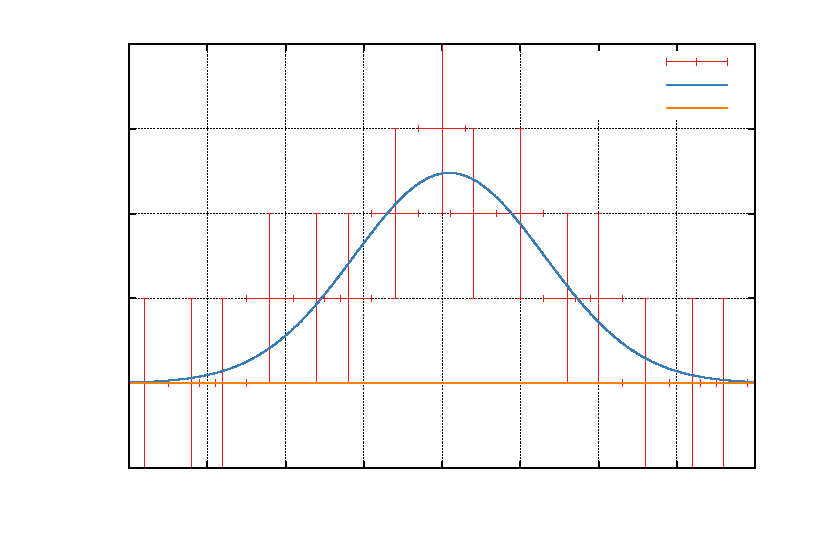
\includegraphics{./plots/aufspaltung/violett2}}%
    \gplfronttext
  \end{picture}%
\endgroup

\caption{nicht sichtbare Isotopieaufspaltung der violetten Balmer-Linien von Wasserstoff und Deuterium}
\label{fig:aufspaltung_violett}
\end{figure}
\FloatBarrier
In Abbildung \ref{fig:aufspaltung_blau} ist offensichtlich, dass die Amplitude der Maxima nicht korrekt angepasst wurde.
Da die Linien sehr schmal und die Aufspaltung sehr gering ist, liegen hier wenige Messdaten vor, an die die Funktion angepasst werden kann.
Dabei ist die Anpassung auch noch sehr stark von der Wahl der Anfangsbedingungen abhängig.
Einzig die für diese Anpassung gewählten Anfangsbedingungen (der Anfangswert der Amplitude des Hauptmaximas wurde bei der Anpassung übernommen) liefert ein halbwegs sinnvolles Ergebnis.
Da die Amplitude zur Auswertung nicht benötigt wird und die Schwerpunkte der Gaußkurven sinnvoll erscheinen, ist dies die unserer Meinung nach beste Möglichkeit, auswertbare Daten zu erhalten und wir werden diese Anpassung zur Auswertung nutzen.

In Tabelle \ref{tab:balmer_ccd_messwerte} sind die Messwerte, die der Auswertung zugrunde liegen, dargestellt.
Die Ergebnisse der Anpassungen durch \texttt{gnuplot} sind dort ebenfalls  in den Spalten "`Schwerpunkt 1"' und "`Schwerpunkt 2"' dargestellt.
Aus der Differenz der Schwerpunkte errechnen wir in \ref{tab:balmer_ccd_auswertung} die Winkelaufspaltung $\Delta\beta$ zwischen der Wasserstoff- und Deuteriumlinie.\\
\\
Aus der Gittergleichung \eqref{eq:gittergleichung} folgt durch Differenzieren
\begin{align*}
\frac{\text{d}\lambda}{\text{d}\beta}=g\,\cos(\beta)
\end{align*}
und wir erhalten nach Umstellen der Gleichung:
\begin{align}
\Delta\lambda=g\,\cos(\beta)\Delta\beta
\label{eq:balmer_wellenlängenaufspaltung}
\end{align}
Mit \eqref{eq:balmer_wellenlängenaufspaltung} können wir damit die Wellenlängenaufspaltung $\Delta\lambda$ der beiden Linien aus der Winkelaufspaltung und dem Reflexionswinkel ausrechnen.
Den Reflexionswinkel $\beta$ erhalten wir gemäß Abbildung \ref{fig:winkelverhaeltnis} und Formel  \eqref{eq:reflexionswinkel} aus den in Tabelle \ref{tab:balmer_ccd_messwerte} eingetragenen Gitterwinkeln bei festem Bankwinkel $\omega_\text{B}$= \SI{150}{\degree}.
Die so gefundenen Werte sind ebenso wie die Fehler bereits in der Tabelle \ref{tab:balmer_ccd_auswertung} eingetragen.
\begin{table}[h]
\centering
\resizebox{\columnwidth}{!}{%
\begin{tabular}{lllll}
	\toprule
	Farbe & Gitterwinkel $\omega_\text{G}$ / \si{\degree} & Wellenlänge $\lambda$ / \si{\nano\metre} & Schwerpunkt 1 / \si{\degree} & Schwerpunkt 2 / \si{\degree} \\
	\midrule
	Rot		& \num{70.5+-0.5} 	& \num{652.8+-4.1} & \num{0.13556+-0.00025} &	\num{0.16529+-0.00204}\\
	Türkis	& \num{53+-0.5}		& \num{487.6+-5.2} & \num{0.07548+-0.00024} &	\num{0.09338+-0.00220}\\
	Blau 	& \num{48+-0.5}		& \num{431.4+-5.4} & \num{0.00980+-0.00090} &	\num{0.02598+-0.00281}\\
	Violett & \num{46+-0.5}		& \num{407.9+-5.5} & n.v. & n.v. \\
	\bottomrule
\end{tabular}}
\caption{Messwerte bei der Beobachtung der Balmer-Linien mit der CCD-Kamera}
\label{tab:balmer_ccd_messwerte}
\end{table}

\begin{table}[h]
\centering
\begin{tabular}{lllll}
	\toprule
	Farbe & Schwerpunkt 1 / \si{\degree} & Schwerpunkt 2 / \si{\degree} & Winkelaufspaltung $\Delta\beta$ / \si{\degree} & Aufspaltung $\Delta\lambda$ \si{\nano\metre}  \\
	\midrule
	Rot & \num{0.13556+-0.00015} &	\num{0.16529+-0.00104} &	\num{0.000519+-0.000018} &	\num{0.1618+-0.0058} \\
	Türkis & \num{0.07548+-0.00014} &	\num{0.09338+-0.00120} &	\num{0.000312+-0.000021} &	\num{0.1179+-0.0080} \\
	Blau & \num{0.00980+-0.00090} &	\num{0.02598+-0.00281} &	\num{0.000282+-0.000051} &	\num{0.1101+-0.0200} \\
	\bottomrule
\end{tabular}
\caption{Auswertung der Balmer-Linien mit der CCD-Kamera}
\label{tab:balmer_ccd_auswertung}
\end{table}
\noindent
Zum Vergleich errechnen wir mit \eqref{eq:rydberg} die folgenden theoretischen Werte:
\begin{align}
\Delta\lambda_\alpha=\SI{0.179}{\nano\metre}\\
\Delta\lambda_\beta=\SI{0.132}{\nano\metre}\\
\Delta\lambda_\gamma=\SI{0.118}{\nano\metre}
\end{align}
Die von uns gemessenen Werte liegen alle unter den theoretischen Werten für die Wellenlängenverschiebung.
Der Literaturwert der roten Balmer-Linie liegt nicht mehr im $1$-$\sigma$-Bereich der gemessenen Isotopieaufspaltung, die anderen beiden Aufspaltungen sind unter Berücksichtigung der Fehlergrenzen mit dem Literaturwert verträglich.
Die Aufspaltung der blauen Linie ist unter Berücksichtigung der schlechten Anpassung, die der Auswertung zugrunde liegt, gut bestimmt worden.
\clearpage


\clearpage

\begin{table}
\centering
\begin{subtable}{0.5\textwidth}
\centering

<tabular-environment>

\caption{<subcaption>}
\end{subtable}%
\begin{subtable}{0.5\textwidth}
\centering

<tabular-environment>

\caption{<subcaption>}
\end{subtable}

\caption{<main caption>}
\end{table}

\section{Grafikstorage}

\begin{figure}
\centering
% GNUPLOT: LaTeX picture with Postscript
\begingroup
  \makeatletter
  \providecommand\color[2][]{%
    \GenericError{(gnuplot) \space\space\space\@spaces}{%
      Package color not loaded in conjunction with
      terminal option `colourtext'%
    }{See the gnuplot documentation for explanation.%
    }{Either use 'blacktext' in gnuplot or load the package
      color.sty in LaTeX.}%
    \renewcommand\color[2][]{}%
  }%
  \providecommand\includegraphics[2][]{%
    \GenericError{(gnuplot) \space\space\space\@spaces}{%
      Package graphicx or graphics not loaded%
    }{See the gnuplot documentation for explanation.%
    }{The gnuplot epslatex terminal needs graphicx.sty or graphics.sty.}%
    \renewcommand\includegraphics[2][]{}%
  }%
  \providecommand\rotatebox[2]{#2}%
  \@ifundefined{ifGPcolor}{%
    \newif\ifGPcolor
    \GPcolortrue
  }{}%
  \@ifundefined{ifGPblacktext}{%
    \newif\ifGPblacktext
    \GPblacktexttrue
  }{}%
  % define a \g@addto@macro without @ in the name:
  \let\gplgaddtomacro\g@addto@macro
  % define empty templates for all commands taking text:
  \gdef\gplbacktext{}%
  \gdef\gplfronttext{}%
  \makeatother
  \ifGPblacktext
    % no textcolor at all
    \def\colorrgb#1{}%
    \def\colorgray#1{}%
  \else
    % gray or color?
    \ifGPcolor
      \def\colorrgb#1{\color[rgb]{#1}}%
      \def\colorgray#1{\color[gray]{#1}}%
      \expandafter\def\csname LTw\endcsname{\color{white}}%
      \expandafter\def\csname LTb\endcsname{\color{black}}%
      \expandafter\def\csname LTa\endcsname{\color{black}}%
      \expandafter\def\csname LT0\endcsname{\color[rgb]{1,0,0}}%
      \expandafter\def\csname LT1\endcsname{\color[rgb]{0,1,0}}%
      \expandafter\def\csname LT2\endcsname{\color[rgb]{0,0,1}}%
      \expandafter\def\csname LT3\endcsname{\color[rgb]{1,0,1}}%
      \expandafter\def\csname LT4\endcsname{\color[rgb]{0,1,1}}%
      \expandafter\def\csname LT5\endcsname{\color[rgb]{1,1,0}}%
      \expandafter\def\csname LT6\endcsname{\color[rgb]{0,0,0}}%
      \expandafter\def\csname LT7\endcsname{\color[rgb]{1,0.3,0}}%
      \expandafter\def\csname LT8\endcsname{\color[rgb]{0.5,0.5,0.5}}%
    \else
      % gray
      \def\colorrgb#1{\color{black}}%
      \def\colorgray#1{\color[gray]{#1}}%
      \expandafter\def\csname LTw\endcsname{\color{white}}%
      \expandafter\def\csname LTb\endcsname{\color{black}}%
      \expandafter\def\csname LTa\endcsname{\color{black}}%
      \expandafter\def\csname LT0\endcsname{\color{black}}%
      \expandafter\def\csname LT1\endcsname{\color{black}}%
      \expandafter\def\csname LT2\endcsname{\color{black}}%
      \expandafter\def\csname LT3\endcsname{\color{black}}%
      \expandafter\def\csname LT4\endcsname{\color{black}}%
      \expandafter\def\csname LT5\endcsname{\color{black}}%
      \expandafter\def\csname LT6\endcsname{\color{black}}%
      \expandafter\def\csname LT7\endcsname{\color{black}}%
      \expandafter\def\csname LT8\endcsname{\color{black}}%
    \fi
  \fi
  \setlength{\unitlength}{0.0500bp}%
  \begin{picture}(7200.00,5040.00)%
    \gplgaddtomacro\gplbacktext{%
      \csname LTb\endcsname%
      \put(946,704){\makebox(0,0)[r]{\strut{} 400}}%
      \csname LTb\endcsname%
      \put(946,1383){\makebox(0,0)[r]{\strut{} 450}}%
      \csname LTb\endcsname%
      \put(946,2061){\makebox(0,0)[r]{\strut{} 500}}%
      \csname LTb\endcsname%
      \put(946,2740){\makebox(0,0)[r]{\strut{} 550}}%
      \csname LTb\endcsname%
      \put(946,3418){\makebox(0,0)[r]{\strut{} 600}}%
      \csname LTb\endcsname%
      \put(946,4097){\makebox(0,0)[r]{\strut{} 650}}%
      \csname LTb\endcsname%
      \put(946,4775){\makebox(0,0)[r]{\strut{} 700}}%
      \csname LTb\endcsname%
      \put(1078,484){\makebox(0,0){\strut{} 0.9}}%
      \csname LTb\endcsname%
      \put(1794,484){\makebox(0,0){\strut{} 1}}%
      \csname LTb\endcsname%
      \put(2509,484){\makebox(0,0){\strut{} 1.1}}%
      \csname LTb\endcsname%
      \put(3225,484){\makebox(0,0){\strut{} 1.2}}%
      \csname LTb\endcsname%
      \put(3941,484){\makebox(0,0){\strut{} 1.3}}%
      \csname LTb\endcsname%
      \put(4656,484){\makebox(0,0){\strut{} 1.4}}%
      \csname LTb\endcsname%
      \put(5372,484){\makebox(0,0){\strut{} 1.5}}%
      \csname LTb\endcsname%
      \put(6087,484){\makebox(0,0){\strut{} 1.6}}%
      \csname LTb\endcsname%
      \put(6803,484){\makebox(0,0){\strut{} 1.7}}%
      \put(176,2739){\rotatebox{-270}{\makebox(0,0){\strut{}Wellenlänge $\lambda$ / \si{\nano\meter}}}}%
      \put(3940,154){\makebox(0,0){\strut{}$\sin(\alpha)+\sin(\beta)$'}}%
      \put(3940,4665){\makebox(0,0){\strut{}}}%
    }%
    \gplgaddtomacro\gplfronttext{%
      \csname LTb\endcsname%
      \put(5816,1097){\makebox(0,0)[r]{\strut{}Messwerte}}%
      \csname LTb\endcsname%
      \put(5816,877){\makebox(0,0)[r]{\strut{}Regressionsgerade}}%
    }%
    \gplbacktext
    \put(0,0){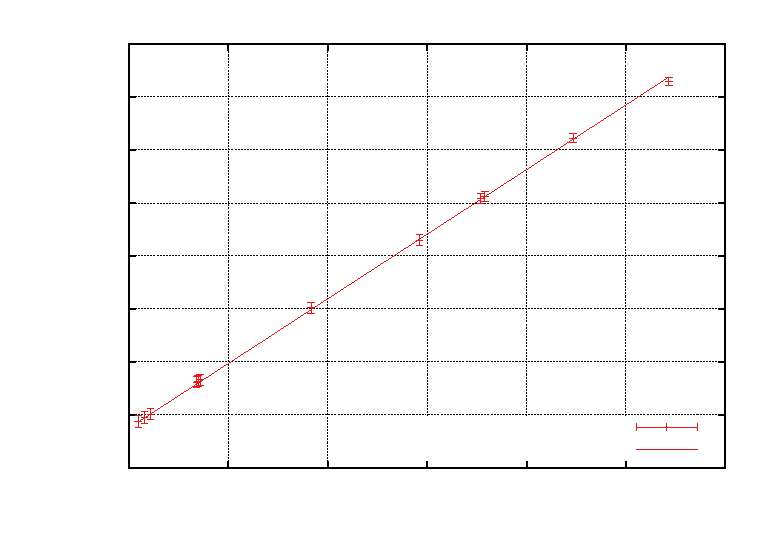
\includegraphics{./plots/gitterkonstante}}%
    \gplfronttext
  \end{picture}%
\endgroup

\caption{Gitterkonstante}
\label{fig:gitterkonstante}
\end{figure}

\clearpage

\begin{figure}
	\centering
	% GNUPLOT: LaTeX picture with Postscript
\begingroup
  \makeatletter
  \providecommand\color[2][]{%
    \GenericError{(gnuplot) \space\space\space\@spaces}{%
      Package color not loaded in conjunction with
      terminal option `colourtext'%
    }{See the gnuplot documentation for explanation.%
    }{Either use 'blacktext' in gnuplot or load the package
      color.sty in LaTeX.}%
    \renewcommand\color[2][]{}%
  }%
  \providecommand\includegraphics[2][]{%
    \GenericError{(gnuplot) \space\space\space\@spaces}{%
      Package graphicx or graphics not loaded%
    }{See the gnuplot documentation for explanation.%
    }{The gnuplot epslatex terminal needs graphicx.sty or graphics.sty.}%
    \renewcommand\includegraphics[2][]{}%
  }%
  \providecommand\rotatebox[2]{#2}%
  \@ifundefined{ifGPcolor}{%
    \newif\ifGPcolor
    \GPcolortrue
  }{}%
  \@ifundefined{ifGPblacktext}{%
    \newif\ifGPblacktext
    \GPblacktexttrue
  }{}%
  % define a \g@addto@macro without @ in the name:
  \let\gplgaddtomacro\g@addto@macro
  % define empty templates for all commands taking text:
  \gdef\gplbacktext{}%
  \gdef\gplfronttext{}%
  \makeatother
  \ifGPblacktext
    % no textcolor at all
    \def\colorrgb#1{}%
    \def\colorgray#1{}%
  \else
    % gray or color?
    \ifGPcolor
      \def\colorrgb#1{\color[rgb]{#1}}%
      \def\colorgray#1{\color[gray]{#1}}%
      \expandafter\def\csname LTw\endcsname{\color{white}}%
      \expandafter\def\csname LTb\endcsname{\color{black}}%
      \expandafter\def\csname LTa\endcsname{\color{black}}%
      \expandafter\def\csname LT0\endcsname{\color[rgb]{1,0,0}}%
      \expandafter\def\csname LT1\endcsname{\color[rgb]{0,1,0}}%
      \expandafter\def\csname LT2\endcsname{\color[rgb]{0,0,1}}%
      \expandafter\def\csname LT3\endcsname{\color[rgb]{1,0,1}}%
      \expandafter\def\csname LT4\endcsname{\color[rgb]{0,1,1}}%
      \expandafter\def\csname LT5\endcsname{\color[rgb]{1,1,0}}%
      \expandafter\def\csname LT6\endcsname{\color[rgb]{0,0,0}}%
      \expandafter\def\csname LT7\endcsname{\color[rgb]{1,0.3,0}}%
      \expandafter\def\csname LT8\endcsname{\color[rgb]{0.5,0.5,0.5}}%
    \else
      % gray
      \def\colorrgb#1{\color{black}}%
      \def\colorgray#1{\color[gray]{#1}}%
      \expandafter\def\csname LTw\endcsname{\color{white}}%
      \expandafter\def\csname LTb\endcsname{\color{black}}%
      \expandafter\def\csname LTa\endcsname{\color{black}}%
      \expandafter\def\csname LT0\endcsname{\color{black}}%
      \expandafter\def\csname LT1\endcsname{\color{black}}%
      \expandafter\def\csname LT2\endcsname{\color{black}}%
      \expandafter\def\csname LT3\endcsname{\color{black}}%
      \expandafter\def\csname LT4\endcsname{\color{black}}%
      \expandafter\def\csname LT5\endcsname{\color{black}}%
      \expandafter\def\csname LT6\endcsname{\color{black}}%
      \expandafter\def\csname LT7\endcsname{\color{black}}%
      \expandafter\def\csname LT8\endcsname{\color{black}}%
    \fi
  \fi
  \setlength{\unitlength}{0.0500bp}%
  \begin{picture}(6480.00,4320.00)%
    \gplgaddtomacro\gplbacktext{%
      \csname LTb\endcsname%
      \put(946,704){\makebox(0,0)[r]{\strut{} 1,4}}%
      \csname LTb\endcsname%
      \put(946,1262){\makebox(0,0)[r]{\strut{} 1,6}}%
      \csname LTb\endcsname%
      \put(946,1821){\makebox(0,0)[r]{\strut{} 1,8}}%
      \csname LTb\endcsname%
      \put(946,2379){\makebox(0,0)[r]{\strut{} 2}}%
      \csname LTb\endcsname%
      \put(946,2938){\makebox(0,0)[r]{\strut{} 2,2}}%
      \csname LTb\endcsname%
      \put(946,3497){\makebox(0,0)[r]{\strut{} 2,4}}%
      \csname LTb\endcsname%
      \put(946,4055){\makebox(0,0)[r]{\strut{} 2,6}}%
      \csname LTb\endcsname%
      \put(1578,484){\makebox(0,0){\strut{} 0,14}}%
      \csname LTb\endcsname%
      \put(2579,484){\makebox(0,0){\strut{} 0,16}}%
      \csname LTb\endcsname%
      \put(3580,484){\makebox(0,0){\strut{} 0,18}}%
      \csname LTb\endcsname%
      \put(4581,484){\makebox(0,0){\strut{} 0,2}}%
      \csname LTb\endcsname%
      \put(5582,484){\makebox(0,0){\strut{} 0,22}}%
      \put(176,2379){\rotatebox{-270}{\makebox(0,0){\strut{}$\frac{1}{\lambda}$ / $\si{\per\micro\metre}$}}}%
      \put(3580,154){\makebox(0,0){\strut{}$\frac{1}{4} - \frac{1}{n^2}$}}%
      \put(3580,3945){\makebox(0,0){\strut{}}}%
    }%
    \gplgaddtomacro\gplfronttext{%
      \csname LTb\endcsname%
      \put(5096,1097){\makebox(0,0)[r]{\strut{}Messwerte}}%
      \csname LTb\endcsname%
      \put(5096,877){\makebox(0,0)[r]{\strut{}Regressionsgerade}}%
    }%
    \gplbacktext
    \put(0,0){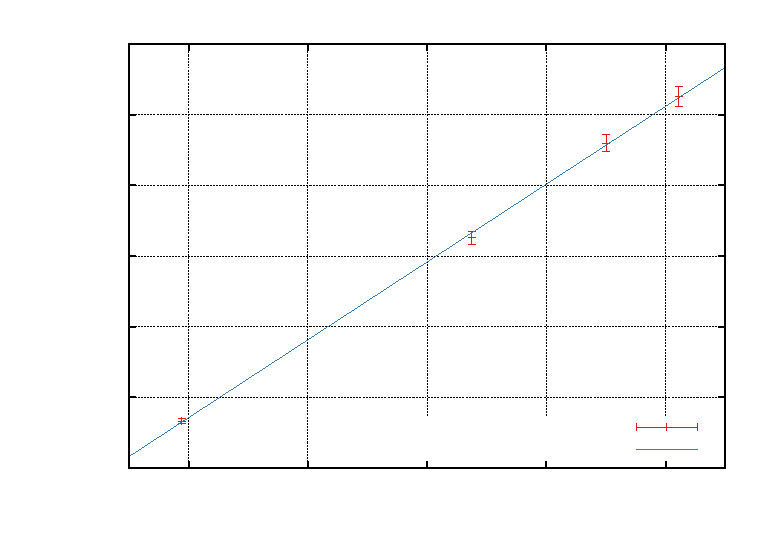
\includegraphics{./plots/rydberg_linearisierung}}%
    \gplfronttext
  \end{picture}%
\endgroup

	\caption{Linearisierung zur Bestimmung der Rydberg-Konstanten}
	\label{fig:rydberg_balmer}
\end{figure}


% BIBLIOGRAPHIE

% Maximale Anzahl der Einträge in Klammer
% Zitieren mit \cite{lamport94}
\begin{thebibliography}{9}

\bibitem{hecht}
	Eugene Hecht,
	\emph{Optik}.
	Oldenbourg,
	5. Auflage
	
\bibitem{siegmann}
	Anthony E. Siegmann,
	\emph{Lasers}.
	University Science Books,
	1986
	
\bibitem{demtroeder3}
	Wolfgang Demtröder,
	\emph{Experimentalphysik 3}.
	Springer Verlag,
	3. Auflage
 
\bibitem{haken_wolf}
	Hermann Haken, Hans Christoph Wolf,
	\emph{Atom- und Quantenphysik}.
	Springer Verlag,
	7. Auflage
 
\end{thebibliography}

% APPENDIX
\begin{appendix}
\section{Anhang}
\subsection{Kennlinien des Photostroms}
\label{app:kennlinien}
\FloatBarrier
% Messung 365nm
\begin{figure}
	\centering
	% GNUPLOT: LaTeX picture with Postscript
\begingroup
  \makeatletter
  \providecommand\color[2][]{%
    \GenericError{(gnuplot) \space\space\space\@spaces}{%
      Package color not loaded in conjunction with
      terminal option `colourtext'%
    }{See the gnuplot documentation for explanation.%
    }{Either use 'blacktext' in gnuplot or load the package
      color.sty in LaTeX.}%
    \renewcommand\color[2][]{}%
  }%
  \providecommand\includegraphics[2][]{%
    \GenericError{(gnuplot) \space\space\space\@spaces}{%
      Package graphicx or graphics not loaded%
    }{See the gnuplot documentation for explanation.%
    }{The gnuplot epslatex terminal needs graphicx.sty or graphics.sty.}%
    \renewcommand\includegraphics[2][]{}%
  }%
  \providecommand\rotatebox[2]{#2}%
  \@ifundefined{ifGPcolor}{%
    \newif\ifGPcolor
    \GPcolortrue
  }{}%
  \@ifundefined{ifGPblacktext}{%
    \newif\ifGPblacktext
    \GPblacktexttrue
  }{}%
  % define a \g@addto@macro without @ in the name:
  \let\gplgaddtomacro\g@addto@macro
  % define empty templates for all commands taking text:
  \gdef\gplbacktext{}%
  \gdef\gplfronttext{}%
  \makeatother
  \ifGPblacktext
    % no textcolor at all
    \def\colorrgb#1{}%
    \def\colorgray#1{}%
  \else
    % gray or color?
    \ifGPcolor
      \def\colorrgb#1{\color[rgb]{#1}}%
      \def\colorgray#1{\color[gray]{#1}}%
      \expandafter\def\csname LTw\endcsname{\color{white}}%
      \expandafter\def\csname LTb\endcsname{\color{black}}%
      \expandafter\def\csname LTa\endcsname{\color{black}}%
      \expandafter\def\csname LT0\endcsname{\color[rgb]{1,0,0}}%
      \expandafter\def\csname LT1\endcsname{\color[rgb]{0,1,0}}%
      \expandafter\def\csname LT2\endcsname{\color[rgb]{0,0,1}}%
      \expandafter\def\csname LT3\endcsname{\color[rgb]{1,0,1}}%
      \expandafter\def\csname LT4\endcsname{\color[rgb]{0,1,1}}%
      \expandafter\def\csname LT5\endcsname{\color[rgb]{1,1,0}}%
      \expandafter\def\csname LT6\endcsname{\color[rgb]{0,0,0}}%
      \expandafter\def\csname LT7\endcsname{\color[rgb]{1,0.3,0}}%
      \expandafter\def\csname LT8\endcsname{\color[rgb]{0.5,0.5,0.5}}%
    \else
      % gray
      \def\colorrgb#1{\color{black}}%
      \def\colorgray#1{\color[gray]{#1}}%
      \expandafter\def\csname LTw\endcsname{\color{white}}%
      \expandafter\def\csname LTb\endcsname{\color{black}}%
      \expandafter\def\csname LTa\endcsname{\color{black}}%
      \expandafter\def\csname LT0\endcsname{\color{black}}%
      \expandafter\def\csname LT1\endcsname{\color{black}}%
      \expandafter\def\csname LT2\endcsname{\color{black}}%
      \expandafter\def\csname LT3\endcsname{\color{black}}%
      \expandafter\def\csname LT4\endcsname{\color{black}}%
      \expandafter\def\csname LT5\endcsname{\color{black}}%
      \expandafter\def\csname LT6\endcsname{\color{black}}%
      \expandafter\def\csname LT7\endcsname{\color{black}}%
      \expandafter\def\csname LT8\endcsname{\color{black}}%
    \fi
  \fi
  \setlength{\unitlength}{0.0500bp}%
  \begin{picture}(6480.00,4320.00)%
    \gplgaddtomacro\gplbacktext{%
      \csname LTb\endcsname%
      \put(946,704){\makebox(0,0)[r]{\strut{} 0}}%
      \csname LTb\endcsname%
      \put(946,1076){\makebox(0,0)[r]{\strut{} 0,5}}%
      \csname LTb\endcsname%
      \put(946,1449){\makebox(0,0)[r]{\strut{} 1}}%
      \csname LTb\endcsname%
      \put(946,1821){\makebox(0,0)[r]{\strut{} 1,5}}%
      \csname LTb\endcsname%
      \put(946,2193){\makebox(0,0)[r]{\strut{} 2}}%
      \csname LTb\endcsname%
      \put(946,2566){\makebox(0,0)[r]{\strut{} 2,5}}%
      \csname LTb\endcsname%
      \put(946,2938){\makebox(0,0)[r]{\strut{} 3}}%
      \csname LTb\endcsname%
      \put(946,3310){\makebox(0,0)[r]{\strut{} 3,5}}%
      \csname LTb\endcsname%
      \put(946,3683){\makebox(0,0)[r]{\strut{} 4}}%
      \csname LTb\endcsname%
      \put(946,4055){\makebox(0,0)[r]{\strut{} 4,5}}%
      \csname LTb\endcsname%
      \put(1078,484){\makebox(0,0){\strut{} 0}}%
      \csname LTb\endcsname%
      \put(2079,484){\makebox(0,0){\strut{} 0,5}}%
      \csname LTb\endcsname%
      \put(3080,484){\makebox(0,0){\strut{} 1}}%
      \csname LTb\endcsname%
      \put(4081,484){\makebox(0,0){\strut{} 1,5}}%
      \csname LTb\endcsname%
      \put(5082,484){\makebox(0,0){\strut{} 2}}%
      \csname LTb\endcsname%
      \put(6083,484){\makebox(0,0){\strut{} 2,5}}%
      \put(176,2379){\rotatebox{-270}{\makebox(0,0){\strut{}$\sqrt{I-I_0} \, / \, \si{\nano\ampere^{1/2}}$}}}%
      \put(3580,154){\makebox(0,0){\strut{}$U \, / \, \si{\volt}$}}%
      \put(3580,3945){\makebox(0,0){\strut{}}}%
    }%
    \gplgaddtomacro\gplfronttext{%
      \csname LTb\endcsname%
      \put(5096,3882){\makebox(0,0)[r]{\strut{}Messung 1}}%
      \csname LTb\endcsname%
      \put(5096,3662){\makebox(0,0)[r]{\strut{}Regressionsgerade 1}}%
      \csname LTb\endcsname%
      \put(5096,3442){\makebox(0,0)[r]{\strut{}Messung 2}}%
      \csname LTb\endcsname%
      \put(5096,3222){\makebox(0,0)[r]{\strut{}Regressionsgerade 2}}%
    }%
    \gplbacktext
    \put(0,0){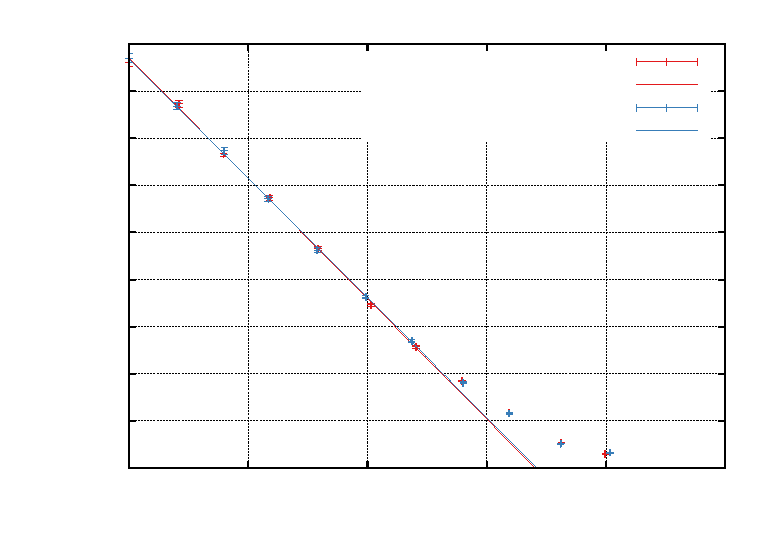
\includegraphics{./plots/photo/kennlinien_365nm}}%
    \gplfronttext
  \end{picture}%
\endgroup

	\caption{Linearisierte Kennlinie zur Grenzspannungsbestimmung $\lambda = \SI{365}{\nano\metre}$}
	\label{fig:kennlinien_365nm}
\end{figure}

\begin{table}
	\centering
	\begin{subtable}{0.5\textwidth}
		\centering
		\vspace{0pt}
		\resizebox{0.95\columnwidth}{!}{%
			\begin{tabular}{SSS}
	\toprule
	{$U$ / \si{\volt}} & {$I-I_0$ / \si{\nano\ampere}} & {$\Delta (I-I_0)$ / \si{\nano\ampere}} \\
	\midrule
0.001 & 18.522 & 0.373 \\
0.209 & 14.922 & 0.301 \\
0.397 & 11.122 & 0.225 \\
0.590 & 8.222  & 0.167 \\
0.793 & 5.422  & 0.111 \\
1.015 & 3.002  & 0.062 \\
1.203 & 1.652  & 0.035 \\
1.395 & 0.852  & 0.019 \\
1.595 & 0.342  & 0.009 \\
1.813 & 0.072  & 0.004 \\
1.997 & 0.022  & 0.003 \\
	\bottomrule
\end{tabular}

		}
		\caption{Messung 1}
	\end{subtable}%
	\begin{subtable}{0.5\textwidth}
		\centering
		\vspace{0pt}
		\resizebox{0.95\columnwidth}{!}{%
			\begin{tabular}{SSS}
	\toprule
	{$U$ / \si{\volt}} & {$I-I_0$ / \si{\nano\ampere}} & {$\Delta (I-I_0)$ / \si{\nano\ampere}} \\
	\midrule
0.001 & 18.927 & 0.381 \\
0.201 & 14.727 & 0.297 \\
0.400 & 11.327 & 0.229 \\
0.583 & 8.167  & 0.165 \\
0.790 & 5.347  & 0.109 \\
0.992 & 3.287  & 0.068 \\
1.185 & 1.817  & 0.038 \\
1.402 & 0.817  & 0.018 \\
1.595 & 0.337  & 0.009 \\
1.810 & 0.067  & 0.003 \\
2.016 & 0.027  & 0.003 \\
	\bottomrule
\end{tabular}

		}
		\caption{Messung 2}
	\end{subtable}

	\caption{Kennlinien der Photozelle f\"ur Licht der Wellenl\"ange $\lambda=\SI{365}{\nano\metre}$}
\end{table}



% Messung 405nm
\begin{figure}
	\centering
	% GNUPLOT: LaTeX picture with Postscript
\begingroup
  \makeatletter
  \providecommand\color[2][]{%
    \GenericError{(gnuplot) \space\space\space\@spaces}{%
      Package color not loaded in conjunction with
      terminal option `colourtext'%
    }{See the gnuplot documentation for explanation.%
    }{Either use 'blacktext' in gnuplot or load the package
      color.sty in LaTeX.}%
    \renewcommand\color[2][]{}%
  }%
  \providecommand\includegraphics[2][]{%
    \GenericError{(gnuplot) \space\space\space\@spaces}{%
      Package graphicx or graphics not loaded%
    }{See the gnuplot documentation for explanation.%
    }{The gnuplot epslatex terminal needs graphicx.sty or graphics.sty.}%
    \renewcommand\includegraphics[2][]{}%
  }%
  \providecommand\rotatebox[2]{#2}%
  \@ifundefined{ifGPcolor}{%
    \newif\ifGPcolor
    \GPcolortrue
  }{}%
  \@ifundefined{ifGPblacktext}{%
    \newif\ifGPblacktext
    \GPblacktexttrue
  }{}%
  % define a \g@addto@macro without @ in the name:
  \let\gplgaddtomacro\g@addto@macro
  % define empty templates for all commands taking text:
  \gdef\gplbacktext{}%
  \gdef\gplfronttext{}%
  \makeatother
  \ifGPblacktext
    % no textcolor at all
    \def\colorrgb#1{}%
    \def\colorgray#1{}%
  \else
    % gray or color?
    \ifGPcolor
      \def\colorrgb#1{\color[rgb]{#1}}%
      \def\colorgray#1{\color[gray]{#1}}%
      \expandafter\def\csname LTw\endcsname{\color{white}}%
      \expandafter\def\csname LTb\endcsname{\color{black}}%
      \expandafter\def\csname LTa\endcsname{\color{black}}%
      \expandafter\def\csname LT0\endcsname{\color[rgb]{1,0,0}}%
      \expandafter\def\csname LT1\endcsname{\color[rgb]{0,1,0}}%
      \expandafter\def\csname LT2\endcsname{\color[rgb]{0,0,1}}%
      \expandafter\def\csname LT3\endcsname{\color[rgb]{1,0,1}}%
      \expandafter\def\csname LT4\endcsname{\color[rgb]{0,1,1}}%
      \expandafter\def\csname LT5\endcsname{\color[rgb]{1,1,0}}%
      \expandafter\def\csname LT6\endcsname{\color[rgb]{0,0,0}}%
      \expandafter\def\csname LT7\endcsname{\color[rgb]{1,0.3,0}}%
      \expandafter\def\csname LT8\endcsname{\color[rgb]{0.5,0.5,0.5}}%
    \else
      % gray
      \def\colorrgb#1{\color{black}}%
      \def\colorgray#1{\color[gray]{#1}}%
      \expandafter\def\csname LTw\endcsname{\color{white}}%
      \expandafter\def\csname LTb\endcsname{\color{black}}%
      \expandafter\def\csname LTa\endcsname{\color{black}}%
      \expandafter\def\csname LT0\endcsname{\color{black}}%
      \expandafter\def\csname LT1\endcsname{\color{black}}%
      \expandafter\def\csname LT2\endcsname{\color{black}}%
      \expandafter\def\csname LT3\endcsname{\color{black}}%
      \expandafter\def\csname LT4\endcsname{\color{black}}%
      \expandafter\def\csname LT5\endcsname{\color{black}}%
      \expandafter\def\csname LT6\endcsname{\color{black}}%
      \expandafter\def\csname LT7\endcsname{\color{black}}%
      \expandafter\def\csname LT8\endcsname{\color{black}}%
    \fi
  \fi
  \setlength{\unitlength}{0.0500bp}%
  \begin{picture}(7200.00,5040.00)%
    \gplgaddtomacro\gplbacktext{%
      \csname LTb\endcsname%
      \put(946,704){\makebox(0,0)[r]{\strut{} 0}}%
      \csname LTb\endcsname%
      \put(946,1383){\makebox(0,0)[r]{\strut{} 0.5}}%
      \csname LTb\endcsname%
      \put(946,2061){\makebox(0,0)[r]{\strut{} 1}}%
      \csname LTb\endcsname%
      \put(946,2740){\makebox(0,0)[r]{\strut{} 1.5}}%
      \csname LTb\endcsname%
      \put(946,3418){\makebox(0,0)[r]{\strut{} 2}}%
      \csname LTb\endcsname%
      \put(946,4097){\makebox(0,0)[r]{\strut{} 2.5}}%
      \csname LTb\endcsname%
      \put(946,4775){\makebox(0,0)[r]{\strut{} 3}}%
      \csname LTb\endcsname%
      \put(1078,484){\makebox(0,0){\strut{} 0}}%
      \csname LTb\endcsname%
      \put(1714,484){\makebox(0,0){\strut{} 0.2}}%
      \csname LTb\endcsname%
      \put(2350,484){\makebox(0,0){\strut{} 0.4}}%
      \csname LTb\endcsname%
      \put(2986,484){\makebox(0,0){\strut{} 0.6}}%
      \csname LTb\endcsname%
      \put(3622,484){\makebox(0,0){\strut{} 0.8}}%
      \csname LTb\endcsname%
      \put(4259,484){\makebox(0,0){\strut{} 1}}%
      \csname LTb\endcsname%
      \put(4895,484){\makebox(0,0){\strut{} 1.2}}%
      \csname LTb\endcsname%
      \put(5531,484){\makebox(0,0){\strut{} 1.4}}%
      \csname LTb\endcsname%
      \put(6167,484){\makebox(0,0){\strut{} 1.6}}%
      \csname LTb\endcsname%
      \put(6803,484){\makebox(0,0){\strut{} 1.8}}%
      \put(176,2739){\rotatebox{-270}{\makebox(0,0){\strut{}$\sqrt{I-I_0} \, / \, \si{\nano\ampere^{1/2}}$}}}%
      \put(3940,154){\makebox(0,0){\strut{}$U \, / \, \si{\volt}$}}%
      \put(3940,4665){\makebox(0,0){\strut{}}}%
    }%
    \gplgaddtomacro\gplfronttext{%
      \csname LTb\endcsname%
      \put(5816,4602){\makebox(0,0)[r]{\strut{}Messung 1}}%
      \csname LTb\endcsname%
      \put(5816,4382){\makebox(0,0)[r]{\strut{}Regressionsgerade 1}}%
      \csname LTb\endcsname%
      \put(5816,4162){\makebox(0,0)[r]{\strut{}Messung 2}}%
      \csname LTb\endcsname%
      \put(5816,3942){\makebox(0,0)[r]{\strut{}Regressionsgerade 2}}%
    }%
    \gplbacktext
    \put(0,0){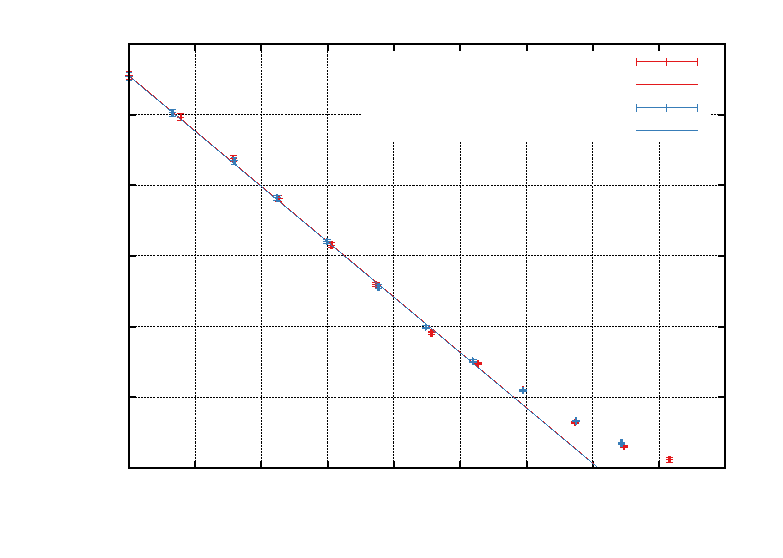
\includegraphics{./plots/photo/kennlinien_405nm}}%
    \gplfronttext
  \end{picture}%
\endgroup

	\caption{Linearisierte Kennlinie zur Grenzspannungsbestimmung $\lambda = \SI{405}{\nano\metre}$}
	\label{fig:kennlinien_405nm}
\end{figure}

\begin{table}
	\centering
	\begin{subtable}{0.5\textwidth}
		\centering
		\vspace{0pt}
		\resizebox{0.95\columnwidth}{!}{%
			\begin{tabular}{SSS}
	\toprule
	{$U$ / \si{\volt}} & {$I-I_0$ / \si{\nano\ampere}} & {$\Delta (I-I_0)$ / \si{\nano\ampere}} \\
	\midrule
0.001 & 7.714 & 0.157 \\
0.156 & 6.164 & 0.126 \\
0.315 & 4.784 & 0.098 \\
0.452 & 3.634 & 0.075 \\
0.611 & 2.484 & 0.052 \\
0.745 & 1.684 & 0.036 \\
0.913 & 0.914 & 0.021 \\
1.053 & 0.544 & 0.013 \\
1.189 & 0.304 & 0.008 \\
1.346 & 0.104 & 0.004 \\
1.494 & 0.024 & 0.003 \\
1.632 & 0.004 & 0.003 \\
	\bottomrule
\end{tabular}

		}
		\caption{Messung 1}
	\end{subtable}%
	\begin{subtable}{0.5\textwidth}
		\centering
		\vspace{0pt}
		\resizebox{0.95\columnwidth}{!}{%
			\begin{tabular}{SSS}
	\toprule
	{$U$ / \si{\volt}} & {$I-I_0$ / \si{\nano\ampere}} & {$\Delta (I-I_0)$ / \si{\nano\ampere}} \\
	\midrule
0.001 & 7.661 & 0.155 \\
0.132 & 6.321 & 0.129 \\
0.318 & 4.721 & 0.097 \\
0.447 & 3.651 & 0.075 \\
0.598 & 2.571 & 0.054 \\
0.753 & 1.641 & 0.035 \\
0.896 & 0.991 & 0.022 \\
1.038 & 0.571 & 0.014 \\
1.189 & 0.301 & 0.008 \\
1.349 & 0.111 & 0.004 \\
1.487 & 0.031 & 0.003 \\
	\bottomrule
\end{tabular}


		}
		\caption{Messung 2}
	\end{subtable}

	\caption{Kennlinien der Photozelle f\"ur Licht der Wellenl\"ange $\lambda = \SI{405}{\nano\metre}$}
\end{table}



% Messung 436nm
\begin{figure}
	\centering
	% GNUPLOT: LaTeX picture with Postscript
\begingroup
  \makeatletter
  \providecommand\color[2][]{%
    \GenericError{(gnuplot) \space\space\space\@spaces}{%
      Package color not loaded in conjunction with
      terminal option `colourtext'%
    }{See the gnuplot documentation for explanation.%
    }{Either use 'blacktext' in gnuplot or load the package
      color.sty in LaTeX.}%
    \renewcommand\color[2][]{}%
  }%
  \providecommand\includegraphics[2][]{%
    \GenericError{(gnuplot) \space\space\space\@spaces}{%
      Package graphicx or graphics not loaded%
    }{See the gnuplot documentation for explanation.%
    }{The gnuplot epslatex terminal needs graphicx.sty or graphics.sty.}%
    \renewcommand\includegraphics[2][]{}%
  }%
  \providecommand\rotatebox[2]{#2}%
  \@ifundefined{ifGPcolor}{%
    \newif\ifGPcolor
    \GPcolortrue
  }{}%
  \@ifundefined{ifGPblacktext}{%
    \newif\ifGPblacktext
    \GPblacktexttrue
  }{}%
  % define a \g@addto@macro without @ in the name:
  \let\gplgaddtomacro\g@addto@macro
  % define empty templates for all commands taking text:
  \gdef\gplbacktext{}%
  \gdef\gplfronttext{}%
  \makeatother
  \ifGPblacktext
    % no textcolor at all
    \def\colorrgb#1{}%
    \def\colorgray#1{}%
  \else
    % gray or color?
    \ifGPcolor
      \def\colorrgb#1{\color[rgb]{#1}}%
      \def\colorgray#1{\color[gray]{#1}}%
      \expandafter\def\csname LTw\endcsname{\color{white}}%
      \expandafter\def\csname LTb\endcsname{\color{black}}%
      \expandafter\def\csname LTa\endcsname{\color{black}}%
      \expandafter\def\csname LT0\endcsname{\color[rgb]{1,0,0}}%
      \expandafter\def\csname LT1\endcsname{\color[rgb]{0,1,0}}%
      \expandafter\def\csname LT2\endcsname{\color[rgb]{0,0,1}}%
      \expandafter\def\csname LT3\endcsname{\color[rgb]{1,0,1}}%
      \expandafter\def\csname LT4\endcsname{\color[rgb]{0,1,1}}%
      \expandafter\def\csname LT5\endcsname{\color[rgb]{1,1,0}}%
      \expandafter\def\csname LT6\endcsname{\color[rgb]{0,0,0}}%
      \expandafter\def\csname LT7\endcsname{\color[rgb]{1,0.3,0}}%
      \expandafter\def\csname LT8\endcsname{\color[rgb]{0.5,0.5,0.5}}%
    \else
      % gray
      \def\colorrgb#1{\color{black}}%
      \def\colorgray#1{\color[gray]{#1}}%
      \expandafter\def\csname LTw\endcsname{\color{white}}%
      \expandafter\def\csname LTb\endcsname{\color{black}}%
      \expandafter\def\csname LTa\endcsname{\color{black}}%
      \expandafter\def\csname LT0\endcsname{\color{black}}%
      \expandafter\def\csname LT1\endcsname{\color{black}}%
      \expandafter\def\csname LT2\endcsname{\color{black}}%
      \expandafter\def\csname LT3\endcsname{\color{black}}%
      \expandafter\def\csname LT4\endcsname{\color{black}}%
      \expandafter\def\csname LT5\endcsname{\color{black}}%
      \expandafter\def\csname LT6\endcsname{\color{black}}%
      \expandafter\def\csname LT7\endcsname{\color{black}}%
      \expandafter\def\csname LT8\endcsname{\color{black}}%
    \fi
  \fi
  \setlength{\unitlength}{0.0500bp}%
  \begin{picture}(7200.00,5040.00)%
    \gplgaddtomacro\gplbacktext{%
      \csname LTb\endcsname%
      \put(946,704){\makebox(0,0)[r]{\strut{} 0}}%
      \csname LTb\endcsname%
      \put(946,1213){\makebox(0,0)[r]{\strut{} 0.5}}%
      \csname LTb\endcsname%
      \put(946,1722){\makebox(0,0)[r]{\strut{} 1}}%
      \csname LTb\endcsname%
      \put(946,2231){\makebox(0,0)[r]{\strut{} 1.5}}%
      \csname LTb\endcsname%
      \put(946,2740){\makebox(0,0)[r]{\strut{} 2}}%
      \csname LTb\endcsname%
      \put(946,3248){\makebox(0,0)[r]{\strut{} 2.5}}%
      \csname LTb\endcsname%
      \put(946,3757){\makebox(0,0)[r]{\strut{} 3}}%
      \csname LTb\endcsname%
      \put(946,4266){\makebox(0,0)[r]{\strut{} 3.5}}%
      \csname LTb\endcsname%
      \put(946,4775){\makebox(0,0)[r]{\strut{} 4}}%
      \csname LTb\endcsname%
      \put(1078,484){\makebox(0,0){\strut{} 0}}%
      \csname LTb\endcsname%
      \put(1794,484){\makebox(0,0){\strut{} 0.2}}%
      \csname LTb\endcsname%
      \put(2509,484){\makebox(0,0){\strut{} 0.4}}%
      \csname LTb\endcsname%
      \put(3225,484){\makebox(0,0){\strut{} 0.6}}%
      \csname LTb\endcsname%
      \put(3941,484){\makebox(0,0){\strut{} 0.8}}%
      \csname LTb\endcsname%
      \put(4656,484){\makebox(0,0){\strut{} 1}}%
      \csname LTb\endcsname%
      \put(5372,484){\makebox(0,0){\strut{} 1.2}}%
      \csname LTb\endcsname%
      \put(6087,484){\makebox(0,0){\strut{} 1.4}}%
      \csname LTb\endcsname%
      \put(6803,484){\makebox(0,0){\strut{} 1.6}}%
      \put(176,2739){\rotatebox{-270}{\makebox(0,0){\strut{}$\sqrt{I-I_0} \, / \, \si{\nano\ampere^{1/2}}$}}}%
      \put(3940,154){\makebox(0,0){\strut{}$U \, / \, \si{\volt}$}}%
      \put(3940,4665){\makebox(0,0){\strut{}}}%
    }%
    \gplgaddtomacro\gplfronttext{%
      \csname LTb\endcsname%
      \put(5816,4602){\makebox(0,0)[r]{\strut{}Messung 1}}%
      \csname LTb\endcsname%
      \put(5816,4382){\makebox(0,0)[r]{\strut{}Regressionsgerade 1}}%
      \csname LTb\endcsname%
      \put(5816,4162){\makebox(0,0)[r]{\strut{}Messung 2}}%
      \csname LTb\endcsname%
      \put(5816,3942){\makebox(0,0)[r]{\strut{}Regressionsgerade 2}}%
    }%
    \gplbacktext
    \put(0,0){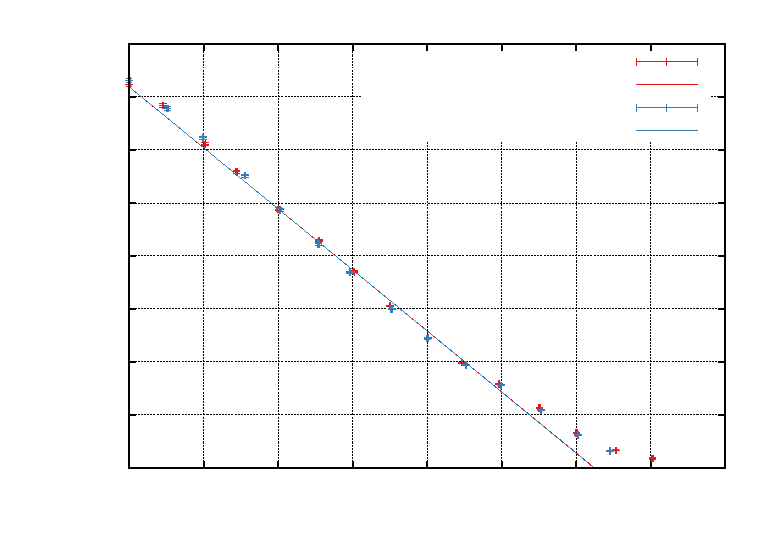
\includegraphics{./plots/photo/kennlinien_436nm}}%
    \gplfronttext
  \end{picture}%
\endgroup

	\caption{Linearisierte Kennlinie zur Grenzspannungsbestimmung $\lambda = \SI{436}{\nano\metre}$}
	\label{fig:kennlinien_436nm}
\end{figure}

\begin{table}
	\centering
	\begin{subtable}{0.5\textwidth}
		\centering
		\vspace{0pt}
		\resizebox{0.95\columnwidth}{!}{%
			\begin{tabular}{SSS}
	\toprule
	{$U$ / \si{\volt}} & {$I-I_0$ / \si{\nano\ampere}} & {$\Delta (I-I_0)$ / \si{\nano\ampere}} \\
	\midrule
0.001 & 13.120 & 0.265 \\
0.091 & 11.708 & 0.237 \\
0.204 & 9.328  & 0.189 \\
0.289 & 7.808  & 0.159 \\
0.401 & 5.958  & 0.122 \\
0.510 & 4.608  & 0.095 \\
0.604 & 3.428  & 0.071 \\
0.700 & 2.338  & 0.049 \\
0.802 & 1.498  & 0.032 \\
0.894 & 0.988  & 0.022 \\
0.993 & 0.628  & 0.015 \\
1.102 & 0.318  & 0.009 \\
1.201 & 0.108  & 0.005 \\
1.306 & 0.028  & 0.003 \\
1.405 & 0.008  & 0.003 \\
	\bottomrule
\end{tabular}

		}
		\caption{Messung 1}
	\end{subtable}%
	\begin{subtable}{0.5\textwidth}
		\centering
		\vspace{0pt}
		\resizebox{0.95\columnwidth}{!}{%
			\begin{tabular}{SSS}
	\toprule
	{$U$ / \si{\volt}} & {$I-I_0$ / \si{\nano\ampere}} & {$\Delta (I-I_0)$ / \si{\nano\ampere}} \\
	\midrule
0.001 & 13.372 & 0.270 \\
0.103 & 11.522 & 0.233 \\
0.199 & 9.712  & 0.196 \\
0.311 & 7.622  & 0.155 \\
0.405 & 5.942  & 0.121 \\
0.508 & 4.482  & 0.092 \\
0.593 & 3.432  & 0.071 \\
0.705 & 2.262  & 0.047 \\
0.801 & 1.512  & 0.032 \\
0.904 & 0.962  & 0.021 \\
0.998 & 0.622  & 0.015 \\
1.106 & 0.312  & 0.008 \\
1.205 & 0.112  & 0.004 \\
1.291 & 0.042  & 0.003 \\
	\bottomrule
\end{tabular}

		}
		\caption{Messung 2}
	\end{subtable}

	\caption{Kennlinien der Photozelle f\"ur Licht der Wellenl\"ange $\lambda = \SI{436}{\nano\metre}$}
\end{table}



% Messung 546nm
\begin{figure}
	\centering
	% GNUPLOT: LaTeX picture with Postscript
\begingroup
  \makeatletter
  \providecommand\color[2][]{%
    \GenericError{(gnuplot) \space\space\space\@spaces}{%
      Package color not loaded in conjunction with
      terminal option `colourtext'%
    }{See the gnuplot documentation for explanation.%
    }{Either use 'blacktext' in gnuplot or load the package
      color.sty in LaTeX.}%
    \renewcommand\color[2][]{}%
  }%
  \providecommand\includegraphics[2][]{%
    \GenericError{(gnuplot) \space\space\space\@spaces}{%
      Package graphicx or graphics not loaded%
    }{See the gnuplot documentation for explanation.%
    }{The gnuplot epslatex terminal needs graphicx.sty or graphics.sty.}%
    \renewcommand\includegraphics[2][]{}%
  }%
  \providecommand\rotatebox[2]{#2}%
  \@ifundefined{ifGPcolor}{%
    \newif\ifGPcolor
    \GPcolortrue
  }{}%
  \@ifundefined{ifGPblacktext}{%
    \newif\ifGPblacktext
    \GPblacktexttrue
  }{}%
  % define a \g@addto@macro without @ in the name:
  \let\gplgaddtomacro\g@addto@macro
  % define empty templates for all commands taking text:
  \gdef\gplbacktext{}%
  \gdef\gplfronttext{}%
  \makeatother
  \ifGPblacktext
    % no textcolor at all
    \def\colorrgb#1{}%
    \def\colorgray#1{}%
  \else
    % gray or color?
    \ifGPcolor
      \def\colorrgb#1{\color[rgb]{#1}}%
      \def\colorgray#1{\color[gray]{#1}}%
      \expandafter\def\csname LTw\endcsname{\color{white}}%
      \expandafter\def\csname LTb\endcsname{\color{black}}%
      \expandafter\def\csname LTa\endcsname{\color{black}}%
      \expandafter\def\csname LT0\endcsname{\color[rgb]{1,0,0}}%
      \expandafter\def\csname LT1\endcsname{\color[rgb]{0,1,0}}%
      \expandafter\def\csname LT2\endcsname{\color[rgb]{0,0,1}}%
      \expandafter\def\csname LT3\endcsname{\color[rgb]{1,0,1}}%
      \expandafter\def\csname LT4\endcsname{\color[rgb]{0,1,1}}%
      \expandafter\def\csname LT5\endcsname{\color[rgb]{1,1,0}}%
      \expandafter\def\csname LT6\endcsname{\color[rgb]{0,0,0}}%
      \expandafter\def\csname LT7\endcsname{\color[rgb]{1,0.3,0}}%
      \expandafter\def\csname LT8\endcsname{\color[rgb]{0.5,0.5,0.5}}%
    \else
      % gray
      \def\colorrgb#1{\color{black}}%
      \def\colorgray#1{\color[gray]{#1}}%
      \expandafter\def\csname LTw\endcsname{\color{white}}%
      \expandafter\def\csname LTb\endcsname{\color{black}}%
      \expandafter\def\csname LTa\endcsname{\color{black}}%
      \expandafter\def\csname LT0\endcsname{\color{black}}%
      \expandafter\def\csname LT1\endcsname{\color{black}}%
      \expandafter\def\csname LT2\endcsname{\color{black}}%
      \expandafter\def\csname LT3\endcsname{\color{black}}%
      \expandafter\def\csname LT4\endcsname{\color{black}}%
      \expandafter\def\csname LT5\endcsname{\color{black}}%
      \expandafter\def\csname LT6\endcsname{\color{black}}%
      \expandafter\def\csname LT7\endcsname{\color{black}}%
      \expandafter\def\csname LT8\endcsname{\color{black}}%
    \fi
  \fi
  \setlength{\unitlength}{0.0500bp}%
  \begin{picture}(7200.00,5040.00)%
    \gplgaddtomacro\gplbacktext{%
      \csname LTb\endcsname%
      \put(946,704){\makebox(0,0)[r]{\strut{} 0}}%
      \csname LTb\endcsname%
      \put(946,1286){\makebox(0,0)[r]{\strut{} 0.5}}%
      \csname LTb\endcsname%
      \put(946,1867){\makebox(0,0)[r]{\strut{} 1}}%
      \csname LTb\endcsname%
      \put(946,2449){\makebox(0,0)[r]{\strut{} 1.5}}%
      \csname LTb\endcsname%
      \put(946,3030){\makebox(0,0)[r]{\strut{} 2}}%
      \csname LTb\endcsname%
      \put(946,3612){\makebox(0,0)[r]{\strut{} 2.5}}%
      \csname LTb\endcsname%
      \put(946,4193){\makebox(0,0)[r]{\strut{} 3}}%
      \csname LTb\endcsname%
      \put(946,4775){\makebox(0,0)[r]{\strut{} 3.5}}%
      \csname LTb\endcsname%
      \put(1078,484){\makebox(0,0){\strut{} 0}}%
      \csname LTb\endcsname%
      \put(1714,484){\makebox(0,0){\strut{} 0.1}}%
      \csname LTb\endcsname%
      \put(2350,484){\makebox(0,0){\strut{} 0.2}}%
      \csname LTb\endcsname%
      \put(2986,484){\makebox(0,0){\strut{} 0.3}}%
      \csname LTb\endcsname%
      \put(3622,484){\makebox(0,0){\strut{} 0.4}}%
      \csname LTb\endcsname%
      \put(4259,484){\makebox(0,0){\strut{} 0.5}}%
      \csname LTb\endcsname%
      \put(4895,484){\makebox(0,0){\strut{} 0.6}}%
      \csname LTb\endcsname%
      \put(5531,484){\makebox(0,0){\strut{} 0.7}}%
      \csname LTb\endcsname%
      \put(6167,484){\makebox(0,0){\strut{} 0.8}}%
      \csname LTb\endcsname%
      \put(6803,484){\makebox(0,0){\strut{} 0.9}}%
      \put(176,2739){\rotatebox{-270}{\makebox(0,0){\strut{}$\sqrt{I-I_0} \, / \, \si{\nano\ampere^{1/2}}$}}}%
      \put(3940,154){\makebox(0,0){\strut{}$U \, / \, \si{\volt}$}}%
      \put(3940,4665){\makebox(0,0){\strut{}}}%
    }%
    \gplgaddtomacro\gplfronttext{%
      \csname LTb\endcsname%
      \put(5816,4602){\makebox(0,0)[r]{\strut{}Messung 1}}%
      \csname LTb\endcsname%
      \put(5816,4382){\makebox(0,0)[r]{\strut{}Regressionsgerade 1}}%
      \csname LTb\endcsname%
      \put(5816,4162){\makebox(0,0)[r]{\strut{}Messung 2}}%
      \csname LTb\endcsname%
      \put(5816,3942){\makebox(0,0)[r]{\strut{}Regressionsgerade 2}}%
    }%
    \gplbacktext
    \put(0,0){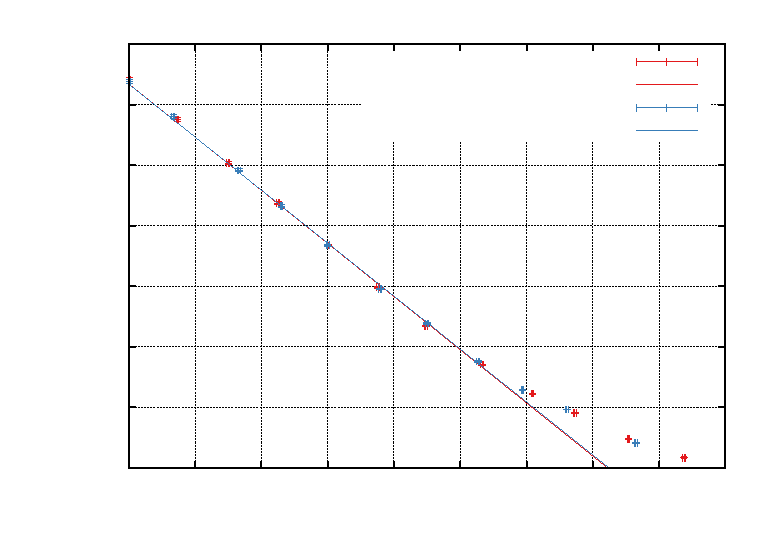
\includegraphics{./plots/photo/kennlinien_546nm}}%
    \gplfronttext
  \end{picture}%
\endgroup

	\caption{Linearisierte Kennlinie zur Grenzspannungsbestimmung $\lambda = \SI{546}{\nano\metre}$}
	\label{fig:kennlinien_546nm}
\end{figure}

\begin{table}
	\centering
	\begin{subtable}{0.5\textwidth}
		\centering
		\vspace{0pt}
		\resizebox{0.95\columnwidth}{!}{%
			\begin{tabular}{SSS}
	\toprule
	{$U$ / \si{\volt}} & {$I-I_0$ / \si{\nano\ampere}} & {$\Delta (I-I_0)$ / \si{\nano\ampere}} \\
	\midrule
0.001 & 10.261 & 0.208 \\
0.073 & 8.261  & 0.168 \\
0.150 & 6.331  & 0.129 \\
0.225 & 4.771  & 0.098 \\
0.301 & 3.371  & 0.070 \\
0.376 & 2.221  & 0.047 \\
0.448 & 1.371  & 0.030 \\
0.533 & 0.721  & 0.017 \\
0.609 & 0.371  & 0.010 \\
0.673 & 0.201  & 0.006 \\
0.754 & 0.051  & 0.003 \\
0.838 & 0.001  & 0.003 \\
	\bottomrule
\end{tabular}

		}
		\caption{Messung 1}
	\end{subtable}%
	\begin{subtable}{0.5\textwidth}
		\centering
		\vspace{0pt}
		\resizebox{0.95\columnwidth}{!}{%
			\begin{tabular}{SSS}
	\toprule
	{$U$ / \si{\volt}} & {$I-I_0$ / \si{\nano\ampere}} & {$\Delta (I-I_0)$ / \si{\nano\ampere}} \\
	\midrule
0.001 & 10.185 & 0.206 \\
0.067 & 8.405  & 0.170 \\
0.166 & 6.035  & 0.123 \\
0.230 & 4.675  & 0.096 \\
0.300 & 3.385  & 0.070 \\
0.379 & 2.185  & 0.046 \\
0.450 & 1.425  & 0.031 \\
0.527 & 0.775  & 0.018 \\
0.594 & 0.415  & 0.011 \\
0.661 & 0.235  & 0.007 \\
0.765 & 0.045  & 0.003 \\
 & & \\
	\bottomrule
\end{tabular}

		}
		\caption{Messung 2}
	\end{subtable}

	\caption{Kennlinien der Photozelle f\"ur Licht der Wellenl\"ange $\lambda = \SI{546}{\nano\metre}$}
\end{table}



% Messung 578nm
\begin{figure}
	\centering
	% GNUPLOT: LaTeX picture with Postscript
\begingroup
  \makeatletter
  \providecommand\color[2][]{%
    \GenericError{(gnuplot) \space\space\space\@spaces}{%
      Package color not loaded in conjunction with
      terminal option `colourtext'%
    }{See the gnuplot documentation for explanation.%
    }{Either use 'blacktext' in gnuplot or load the package
      color.sty in LaTeX.}%
    \renewcommand\color[2][]{}%
  }%
  \providecommand\includegraphics[2][]{%
    \GenericError{(gnuplot) \space\space\space\@spaces}{%
      Package graphicx or graphics not loaded%
    }{See the gnuplot documentation for explanation.%
    }{The gnuplot epslatex terminal needs graphicx.sty or graphics.sty.}%
    \renewcommand\includegraphics[2][]{}%
  }%
  \providecommand\rotatebox[2]{#2}%
  \@ifundefined{ifGPcolor}{%
    \newif\ifGPcolor
    \GPcolortrue
  }{}%
  \@ifundefined{ifGPblacktext}{%
    \newif\ifGPblacktext
    \GPblacktexttrue
  }{}%
  % define a \g@addto@macro without @ in the name:
  \let\gplgaddtomacro\g@addto@macro
  % define empty templates for all commands taking text:
  \gdef\gplbacktext{}%
  \gdef\gplfronttext{}%
  \makeatother
  \ifGPblacktext
    % no textcolor at all
    \def\colorrgb#1{}%
    \def\colorgray#1{}%
  \else
    % gray or color?
    \ifGPcolor
      \def\colorrgb#1{\color[rgb]{#1}}%
      \def\colorgray#1{\color[gray]{#1}}%
      \expandafter\def\csname LTw\endcsname{\color{white}}%
      \expandafter\def\csname LTb\endcsname{\color{black}}%
      \expandafter\def\csname LTa\endcsname{\color{black}}%
      \expandafter\def\csname LT0\endcsname{\color[rgb]{1,0,0}}%
      \expandafter\def\csname LT1\endcsname{\color[rgb]{0,1,0}}%
      \expandafter\def\csname LT2\endcsname{\color[rgb]{0,0,1}}%
      \expandafter\def\csname LT3\endcsname{\color[rgb]{1,0,1}}%
      \expandafter\def\csname LT4\endcsname{\color[rgb]{0,1,1}}%
      \expandafter\def\csname LT5\endcsname{\color[rgb]{1,1,0}}%
      \expandafter\def\csname LT6\endcsname{\color[rgb]{0,0,0}}%
      \expandafter\def\csname LT7\endcsname{\color[rgb]{1,0.3,0}}%
      \expandafter\def\csname LT8\endcsname{\color[rgb]{0.5,0.5,0.5}}%
    \else
      % gray
      \def\colorrgb#1{\color{black}}%
      \def\colorgray#1{\color[gray]{#1}}%
      \expandafter\def\csname LTw\endcsname{\color{white}}%
      \expandafter\def\csname LTb\endcsname{\color{black}}%
      \expandafter\def\csname LTa\endcsname{\color{black}}%
      \expandafter\def\csname LT0\endcsname{\color{black}}%
      \expandafter\def\csname LT1\endcsname{\color{black}}%
      \expandafter\def\csname LT2\endcsname{\color{black}}%
      \expandafter\def\csname LT3\endcsname{\color{black}}%
      \expandafter\def\csname LT4\endcsname{\color{black}}%
      \expandafter\def\csname LT5\endcsname{\color{black}}%
      \expandafter\def\csname LT6\endcsname{\color{black}}%
      \expandafter\def\csname LT7\endcsname{\color{black}}%
      \expandafter\def\csname LT8\endcsname{\color{black}}%
    \fi
  \fi
  \setlength{\unitlength}{0.0500bp}%
  \begin{picture}(7200.00,5040.00)%
    \gplgaddtomacro\gplbacktext{%
      \csname LTb\endcsname%
      \put(946,704){\makebox(0,0)[r]{\strut{} 0}}%
      \csname LTb\endcsname%
      \put(946,1518){\makebox(0,0)[r]{\strut{} 0.5}}%
      \csname LTb\endcsname%
      \put(946,2332){\makebox(0,0)[r]{\strut{} 1}}%
      \csname LTb\endcsname%
      \put(946,3147){\makebox(0,0)[r]{\strut{} 1.5}}%
      \csname LTb\endcsname%
      \put(946,3961){\makebox(0,0)[r]{\strut{} 2}}%
      \csname LTb\endcsname%
      \put(946,4775){\makebox(0,0)[r]{\strut{} 2.5}}%
      \csname LTb\endcsname%
      \put(1078,484){\makebox(0,0){\strut{} 0}}%
      \csname LTb\endcsname%
      \put(1794,484){\makebox(0,0){\strut{} 0.1}}%
      \csname LTb\endcsname%
      \put(2509,484){\makebox(0,0){\strut{} 0.2}}%
      \csname LTb\endcsname%
      \put(3225,484){\makebox(0,0){\strut{} 0.3}}%
      \csname LTb\endcsname%
      \put(3941,484){\makebox(0,0){\strut{} 0.4}}%
      \csname LTb\endcsname%
      \put(4656,484){\makebox(0,0){\strut{} 0.5}}%
      \csname LTb\endcsname%
      \put(5372,484){\makebox(0,0){\strut{} 0.6}}%
      \csname LTb\endcsname%
      \put(6087,484){\makebox(0,0){\strut{} 0.7}}%
      \csname LTb\endcsname%
      \put(6803,484){\makebox(0,0){\strut{} 0.8}}%
      \put(176,2739){\rotatebox{-270}{\makebox(0,0){\strut{}$\sqrt{I-I_0} \, / \, \si{\nano\ampere^{1/2}}$}}}%
      \put(3940,154){\makebox(0,0){\strut{}$U \, / \, \si{\volt}$}}%
      \put(3940,4665){\makebox(0,0){\strut{}}}%
    }%
    \gplgaddtomacro\gplfronttext{%
      \csname LTb\endcsname%
      \put(5816,4602){\makebox(0,0)[r]{\strut{}Messung 1}}%
      \csname LTb\endcsname%
      \put(5816,4382){\makebox(0,0)[r]{\strut{}Regressionsgerade 1}}%
      \csname LTb\endcsname%
      \put(5816,4162){\makebox(0,0)[r]{\strut{}Messung 2}}%
      \csname LTb\endcsname%
      \put(5816,3942){\makebox(0,0)[r]{\strut{}Regressionsgerade 2}}%
    }%
    \gplbacktext
    \put(0,0){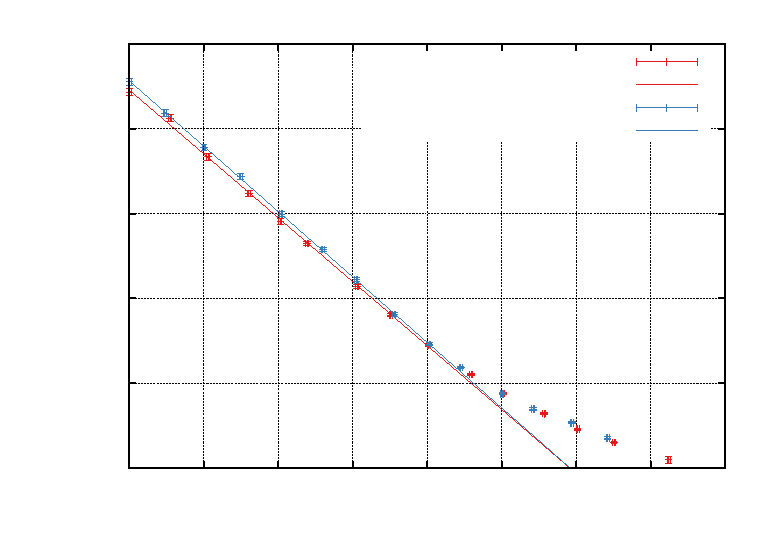
\includegraphics{./plots/photo/kennlinien_578nm}}%
    \gplfronttext
  \end{picture}%
\endgroup

	\caption{Linearisierte Kennlinie zur Grenzspannungsbestimmung $\lambda = \SI{578}{\nano\metre}$}
	\label{fig:kennlinien_578nm}
\end{figure}

\begin{table}
	\centering
	\begin{subtable}{0.5\textwidth}
		\centering
		\vspace{0pt}
		\resizebox{0.95\columnwidth}{!}{%
			\begin{tabular}{SSS}
	\toprule
	{$U$ / \si{\volt}} & {$I-I_0$ / \si{\nano\ampere}} & {$\Delta (I-I_0)$ / \si{\nano\ampere}} \\
	\midrule
0.001 & 4.913 & 0.101 \\
0.055 & 4.253 & 0.087 \\
0.106 & 3.363 & 0.070 \\
0.161 & 2.623 & 0.055 \\
0.203 & 2.113 & 0.045 \\
0.239 & 1.753 & 0.037 \\
0.306 & 1.143 & 0.025 \\
0.351 & 0.813 & 0.019 \\
0.402 & 0.523 & 0.013 \\
0.459 & 0.303 & 0.008 \\
0.502 & 0.193 & 0.006 \\
0.557 & 0.103 & 0.004 \\
0.602 & 0.053 & 0.003 \\
0.651 & 0.023 & 0.003 \\
0.724 & 0.003 & 0.003 \\
	\bottomrule
\end{tabular}

		}
		\caption{Messung 1}
	\end{subtable}%
	\begin{subtable}{0.5\textwidth}
		\centering
		\vspace{0pt}
		\resizebox{0.95\columnwidth}{!}{%
			\begin{tabular}{SSS}
	\toprule
	{$U$ / \si{\volt}} & {$I-I_0$ / \si{\nano\ampere}} & {$\Delta (I-I_0)$ / \si{\nano\ampere}} \\
	\midrule
0.001 & 5.181 & 0.106 \\
0.048 & 4.371 & 0.090 \\
0.101 & 3.571 & 0.074 \\
0.150 & 2.951 & 0.061 \\
0.204 & 2.241 & 0.047 \\
0.260 & 1.661 & 0.036 \\
0.305 & 1.231 & 0.027 \\
0.356 & 0.821 & 0.019 \\
0.403 & 0.531 & 0.013 \\
0.445 & 0.351 & 0.009 \\
0.501 & 0.191 & 0.006 \\
0.542 & 0.121 & 0.005 \\
0.594 & 0.071 & 0.004 \\
0.642 & 0.031 & 0.003 \\
 & & \\
	\bottomrule
\end{tabular}

		}
		\caption{Messung 2}
	\end{subtable}

	\caption{Kennlinien der Photozelle f\"ur Licht der Wellenl\"ange $\lambda = \SI{578}{\nano\metre}$}
\end{table}




\end{appendix}

\end{document}
